\documentclass[12pt,a4paper]{scrartcl}
\usepackage{forest}
\usepackage{booktabs}
\usepackage[breaklinks=true]{hyperref}
\usepackage{placeins}
\usepackage{titling}
\usepackage{graphicx}
\usepackage{listings}
\graphicspath{{figures/}{../figures/}}
\renewcommand{\subtitle}[1]{%
  \posttitle{%
    \par\end{center}
    \begin{center}\large#1\end{center}
    \vskip0.5em}%
}
\title{Laminar EEG-fMRI pipeline}
\author{Tommy Clausner}
\subtitle{\textsc{Documentation}}
\date{\small{last updated on \today}}

\begin{document}
\begin{titlepage}
\clearpage\maketitle
\thispagestyle{empty}
\end{titlepage}
\tableofcontents
\newpage
\listoffigures
\newpage
\listoftables
\newpage
\section{About this Document}
\label{sec:about}
This documententation accompanies the scripts that I wrote for my MSc thesis on feature specific neuronal oscillations on a cortical laminar level under the supervision of:
\begin{itemize}
  \item Mathilde Bonnefond
  \item Rene Scheeringa
\end{itemize}
Hence all the functionality is tied to our specific experiment. However, most steps still can serve as a template for laminar EEG-fMRI analyses in general.\\
\noindent Our experiment consisted of 3 major parts: retinotopic field mapping for visual ROI definition, odd ball task employing gabbor patches (main task) and additional support scans as there are: T1 anatomical and functional scans with inversed flip angle. During the main task EEG was recorded in a $3~s$ gap between blocks of $4~TR$ (4 functional volumes). This led to a signal drop off over each of the four fMRI volumes, that was absent during retinotopy scans. We exploited the fact that the difference between the 4th and 1st volume of such a block yields a T1-like contrast, to optimise co-registration performance.\\
\noindent To enable myself to write all the scripts I got help from various people, so further thanks goes to:
\begin{itemize}
  \item Jose Marques
  \item Koen Haak
  \item Matthias Ekman
  \item Simon Hom\"olle
  \item Tim van Mourik
  \item TG guys at the DCCN
\end{itemize}
The goal was to create a set of scripts such that it would be highly standardized and with as little human interaction as possible. This way it is guaranteed, that once the analysis and respective parameters are set up, the scripts will run similar for all subjects. However it also means that changing single scripts within this "ecosystem" should be done very carefully to not interfere with relative paths and file I/O all functions rely on.
\section{Before starting}
Most of the functionality is optimized for the IT infrastructure provided by the Donders Center for Cognitive Neuroimaging. Since some parts of the analysis require very high amounts of memory, those parts are absolutely infeasible to compute on a local desktop or laptop machine. Given the infrastructure of the DCCN, all scripts were optimized to a reasonable amount for a reduction in computation time but still keeping high spatial accuracy. Hence parts might need to be adjusted to either a different cluster computing system or scaled down massively.\\
All scripts as we used them can be found at \href{https://github.com/TommyClausner/laminarfMRI}{\nolinkurl{https://github.com/TommyClausner/laminarfMRI}}
or by cloning the GitHub repository via the command line:
\begin{lstlisting}[
    language=Shell,
    basicstyle=\ttfamily,
    breaklines=true]
    # download scripts
    git clone https://github.com/TommyClausner/laminarfMRI
\end{lstlisting}
\subsection{Pre- requisites}
\label{sec:prereq}
The present pipeline makes use of many modern state of the art analysis toolboxes for Shell and or MATLAB scripting:
\begin{itemize}
\item analysePRF (\href{http://kendrickkay.net/analyzePRF/}{\nolinkurl{http://kendrickkay.net/analyzePRF/}})
\item FieldTrip (\href{https://github.com/fieldtrip/fieldtrip}{\nolinkurl{https://github.com/fieldtrip/fieldtrip}})
\item FreeSurfer (\href{https://surfer.nmr.mgh.harvard.edu/}{\nolinkurl{https://surfer.nmr.mgh.harvard.edu/}})
\item FSL (\href{https://fsl.fmrib.ox.ac.uk/fsl/fslwiki}{\nolinkurl{https://fsl.fmrib.ox.ac.uk/fsl/fslwiki}})
\item knkutils (\href {https://github.com/kendrickkay/knkutils/}{\nolinkurl{https://github.com/kendrickkay/knkutils/}})
\item MATLAB R2015a or later (\href{https://nl.mathworks.com/products/matlab.html}{\nolinkurl{https://nl.mathworks.com/products/matlab.html}})
\item MRIcron (\href{https://www.nitrc.org/projects/mricron}{\nolinkurl{https://www.nitrc.org/projects/mricron}})
\item Open fMRI Analysis (\href{https://github.com/TimVanMourik/OpenFmriAnalysis}{\nolinkurl{https://github.com/TimVanMourik/OpenFmriAnalysis}})
\item Pipeline (\href{https://github.com/Washington-University/Pipeline}{\nolinkurl{https://github.com/Washington-University/Pipeline}})
\item SPM (\href{http://www.fil.ion.ucl.ac.uk/spm/}{\nolinkurl{http://www.fil.ion.ucl.ac.uk/spm/}})
\item tc\_functions  (\href{https://github.com/TommyClausner/tc\_functions}{\nolinkurl{https://github.com/TommyClausner/tc\_functions}})
\item Tommy's Scriptinator 3000 TM (optional; \href{https://github.com/TommyClausner/Scriptinator}{\nolinkurl{https://github.com/TommyClausner/Scriptinator}})
\item VistaSoft (\href{https://github.com/vistalab/vistasoft}{\nolinkurl{https://github.com/vistalab/vistasoft}})
\item Workbench (\href{https://github.com/Washington-University/Workbench}{\nolinkurl{https://github.com/Washington-University/Workbench}})
\end{itemize}

\noindent Use e.g. MRIcron's dicom2nii to convert raw MRI data to NifTi files.\\

\noindent Call the function "getToolboxes.sh" to download (most of) the software automatically into a folder called toolboxes/ located in the folder from where the function was called (see Section~\ref{sec:getTools} and Figure~\ref{tree:folderstruct})\\
\begin{lstlisting}[
    language=Shell,
    basicstyle=\ttfamily,
    breaklines=true]
    # download toolboxes
    sh getToolboxes.sh
\end{lstlisting}

\subsection{Folder structure}
\label{sec:dirstruct}
The general folder structure is set up by a call to setupfolders.sh (see also Figure \ref{tree:folderstruct}). Raw data should be placed in the corresponding subfolder:
\begin{itemize}
\item Functional data must be located in rawData/niftis/\textbf{functionals}/
\item Anatomical data must be located in in rawData/niftis/\textbf{t1}/
\item Inverted functional data must be located in in rawData/niftis/\textbf{inverted}/
\item Proton density data must be located in in rawData/niftis/\textbf{pd}/
\item Inverted proton density data must be located in in rawData/niftis/\textbf{pdinverted}/
\item EEG data must be located in rawData/\textbf{eegfiles}/
\item Eye tracking data must be located in rawData/\textbf{eyetrackerfiles}/
\item EEG sensor position related files must be in rawData/\textbf{electrodes}/
\item electromagnetic digitizer data must be in rawData/electrodes/\textbf{polhemus}/
\item photogrammetry data must be in rawData/electrodes/\textbf{photogrammetry}/ (note also the respective sub-structure, set up by setupfolders.sh)
\end{itemize}

\subsection{How things work}
Parts of the analysis run in Bash scripts. Those should be called from their root directory using:
\begin{lstlisting}[
    language=Shell,
    basicstyle=\ttfamily,
    breaklines=true]
    # run scripts
    sh scriptname.sh
\end{lstlisting}
Each step within the analysis has a different subfolder containing the respective results of this step. Leading numbers indicate in which logical order the corresponding shell scripts should be executed. Note that all files created by each respective step are stored in the corresponding folder. However files that need to be preset (e.g. config files) must be located in A\_helperfiles. Note Further, that the entire analysis can be broken down to a few sub-pipelines.\\

\noindent Since most operations can be grouped into bigger chunks or "pipelines", all subsections below are wrapped into pipeline scripts, calling them in the respective order. Addtionally a file having the extension .pipe stores the pipeline information in a format readable with Tommy's Scriptinator 3000 TM. This is a java based tool, that can be used to represent and store scripts and their dependencies including a graphical representation. See Section~\ref{sec:scriptinator} of this document of \href{https://github.com/TommyClausner/Scriptinator}{\nolinkurl{https://github.com/TommyClausner/Scriptinator}} for more information.\\

\noindent Further note, that most EEG related scripts rely on MATLAB and FieldTrip. Those scripts can be run stand-alone inside MATLAB or using the bash-script wrapper that has the exact same name only with the file extension .sh instead of .m Furthermore some MATLAB scipts require significant computation time, for which reason they are set up to be run as parts of a whole. In this case the words \textit{split} is added to the file name. Those scripts call the corresponding shell scripts that call the MATLAB scripts in turn, in a organized manner to be run on the cluster.\\

\noindent When using such a MATLAB wrapper some MATLAB language specific details and variables are added to the base-file (targetScript.m). In every case the respective absolute folder path is provided. The shell script creates a temporary file and run it. It will be constructed by adding variables to an empty file and afterwards adding the actual base-file like so:
\begin{lstlisting}[
    language=Shell,
    basicstyle=\ttfamily,
    breaklines=true]
    # guts of MATLAB wrapper
    DIR="$( cd "$( dirname "${BASH_SOURCE[0]}" )" && pwd )"
    cd $DIR
    nameadd=$(date +"%m%d%Y%H%M%S")
    echo "mainpath=" "'$DIR';">$DIR/tmp_$nameadd.m
    cat $DIR/targetScript.m>>$DIR/tmp_$nameadd.m
    echo 'matlab2017b -nosplash -r "run('"'"$DIR/tmp_$nameadd.m"'"');"'  | qsub -q $jobtype -l walltime=$walltime,mem=$memory
\end{lstlisting}

\section{Helper files}
There are several helper files that are needed in order to perform the analysis:

\subsection{acquisition\_parameters.txt}
indicating the respective acquisition parameters per volume needed in order to perform the distortion correction. One line indicates the respective parameter setting for the respective volume (1st line corresponds to 1st volume, etc.)\\

\noindent e.g.:

\noindent 0 1 0 0.042\\
\noindent 0 -1 0 0.042\\

The first 3 columns indicate the respective phase coding direction the last column some weird value, that is only important if it changes. Otherwise it's fine to use any value as long as it is the same.

\subsection{b02b0.cnf}
Settings for distortion correction.

Needed in order to set the parameters for the distortion correction (example provided by FSL). For more information see \href{https://fsl.fmrib.ox.ac.uk/fsl/fslwiki/topup/TopupUsersGuide/}{\nolinkurl{https://fsl.fmrib.ox.ac.uk/fsl/fslwiki/topup/TopupUsersGuide/}}.

\subsection{params.mat}
Parameters used for retinotopy scans as obtained from VistaDisp. For more information see \href{https://web.stanford.edu/group/vista/cgi-bin/wiki/index.php/Stimulus}{\nolinkurl{https://web.stanford.edu/group/vista/cgi-bin/wiki/index.php/Stimulus}}.

\subsection{images.mat}
Stimuli used for retinotopy scans. Stimuli file must be such that each frame is represented as a binary image. The matrix must be of shape $Y \times X \times T$ where $X$ and $Y$ are the image dimensions in pixel and T is the respective number of frames.

\section{qsub}
Scripts that are flagged with the (Q) can be submitted as a qsub job.

\noindent When running the computation on the cluster use the wrapper function runonqsub.sh like so
\begin{lstlisting}[
    language=Shell,
    basicstyle=\ttfamily,
    breaklines=true]
    # run scripts on cluster using wrapper function
    sh runonqsub.sh 32gb targetScript.sh
\end{lstlisting}


\noindent Note that some scripts send a MATLAB script to the qsub cluster. Thus they cannot be run using runonqsub.sh, but instead create their own job. However those scripts can also run stand-alone within a interactive MATLAB session.\\

\noindent Some scripts are present as scriptnameQsub.sh Those scripts contain an internal Qsub-wrapper and do the same as sh runonqsub.sh XXgb scriptname.sh Those scripts are created when using Pipelines (see Section~\ref{sec:pipelines}).\\

\noindent Table~\ref{tab:hardwarerequirements} gives an overview about requirements on memory and computation time can be expected:

\begin{table}[h]
\centering
\begin{tabular}{l | r | l}
\toprule
script & memory required & time required\\\hline
	do\_preparefunctionals.sh & 32GB & $\approx 10min$ \\\hline
  do\_realignment.sh & 32GB & $\approx 30min$ \\\hline
  do\_distcorr.sh & 32GB & $\approx 15min$ \\\hline
  do\_applysimpledistcorr.sh & 32GB & $\approx 30min$ \\\hline
  do\_preparecoregistration.sh & 16GB & $\approx 4.5h$ \\\hline
  do\_correctavgdiff.sh & 4GB & $\approx 3sec$ \\\hline
	do\_fsrecon.sh & 16GB & $\approx 6h$ \\\hline
  do\_coregistration.sh & 16GB & $\approx 30min$ \\\hline
	do\_makemasksandlabels.sh & 16GB & $\approx 1min$ \\\hline
	do\_tseriesinterpolation.sh & 64GB & $\approx 20min$ \\\hline
	do\_split\_analyzePRF.sh & 480GB & $\approx 7h$ \\\hline
  do\_analyzePRF.sh & 6GB & $\approx 7h$ \\\hline
	combine\_split\_PRF\_results.sh & 64GB & $\approx 10min$ \\\hline
  make\_PRF\_overlays.sh & 16GB & $\approx 10min$ \\\hline
	makeOverlays.sh & 16GB & $\approx 5min$\\\hline
	GUI2ROIs.sh & 8GB & user dependent \\\hline
  labels2masks.sh & 8GB & $\approx 10s$ \\\hline
  expandROIs.sh & 16GB & $\approx 3min$ \\\hline
  do\_getLayers.sh & 16GB & $\approx 20min$ \\\hline
  do\_getLayerWeights.sh & 16GB & $\approx 5min$ \\\hline
  do\_EEGpreprocessing.sh & 16GB & $\approx 30min$ \\\hline
  do\_EEGprepareFS.sh & 8GB & $\approx XXXmin$ \\\hline
  do\_EEGprepareHeadmodel.sh & 32GB & $\approx XXXmin$ \\\hline
  do\_EEGelectrodeRegistration.sh & 16GB & user dependent \\\hline
  do\_EEGprepareSourcemodel.sh & 32GB & $\approx XXXmin$ \\\hline
  do\_EEGtimelock.sh & 16GB & $\approx 5min$ \\\hline
  do\_EEGsplitBeamformer.sh & 480GB & $\approx 5h$ \\\hline
  do\_EEGbeamformer.sh & 60GB & $\approx 5h$ \\\hline
  do\_EEGsplitVirtualChannel.sh & 240GB & $\approx 5h$ \\\hline
  do\_EEGvirtualChannel.sh & 30GB & $\approx 5h$ \\\hline
  do\_EEGsplitFreqOnVirtChan.sh & 960GB & $\approx 5h$ \\\hline
  do\_EEGfreqOnVirtChan.sh & 60GB & $\approx 5h$ \\\hline
  do\_EEGfreqChanSelect.sh & 256GB & $\approx 30min$ \\\bottomrule
\end{tabular}
\caption[Approximated time and memory requirements when running on qsub]{Approximated time and memory requirements for the respective script to run. Note that everything that is more than 4GB should be run on the cluster. Use runonqsub.sh or the respective MATLAB wrapper for that purpose.}
\label{tab:hardwarerequirements}
\end{table}

\newpage
\begin{figure}
\caption{Initial folder structure as required for the analysis}
\vspace{10pt}
{\scriptsize
\begin{forest}
  for tree={
    font=\ttfamily,
    grow'=0,
    child anchor=west,
    text height=0.01cm,
    parent anchor=south,
    anchor=west,
    calign=first,
    edge path={
      \noexpand\path [draw, \forestoption{edge}]
      (!u.south west) +(12pt,0pt) |- node[fill,inner sep=1.25pt] {} (.child anchor)\forestoption{edge label};
    },
    before typesetting nodes={
      if n=1
        {insert before={[,phantom]}}
        {}
    },
    fit=band,
    before computing xy={l=20pt},
  }
  [Analysis folder
[toolboxes/
    [see Section \ref{sec:prereq}]
  ]
[S\#/ (set up by setupfolders.sh or when created using makenewsubject.sh)
  [0\_freesurfer/
  ]
  [1\_realignment/
  ]
  [2\_coregistration/
  ]
  [3\_distcorrection/
  ]
  [4\_retinotopy/
  ]
  [5\_laminar/
  ]
  [6\_EEG/
  ]
  [A\_helperfiles/
    [acquisition\_parameters.txt]
    [b02b0.cnf]
    [params.mat]
    [images.mat]
  ]
  [B\_scripts/
    [*.m]
    [*.pipe]
    [*.sh]
  ]
  [C\_miscResults/
  ]
    [rawData/
      [niftis/
      [functionals/]
      [inverted/]
      [pd/]
      [pdinverted/]
      [t1/]
      ]
      [eegfiles/]
      [electrodes/
        [photogrammetry/
          [3Dobject/]
          [photographs/
            [masks/]
          ]
          [photoscanfiles/]
        ]
        [polhemus/]
      ]
      [eyetrackerfiles/]
    ]
]
[template\_session/
[template\_helperfiles/
	[acquisition\_parameters.txt]
  [b02b0.cnf]
  [b02b0\_example\_fsl.cnf]
  [params.mat]
  [images.mat]
]
[template\_scripts/
	[*.m]
  [*.pipe]
  [*.sh]
]
]
[makenewsubject.sh]
[getToolboxes.sh]
]
\end{forest}

}
\label{tree:folderstruct}
\end{figure}

\FloatBarrier

\section{Quick Start}
This document builds upon the analysis rational used during our own analyses. It is build upon the technically facilities of the DCCN (Radboud University Nijmegen, 2018). Hence a copy-paste workflow will only work on a very similar infrastructure.\\
\subsection{first steps}
\begin{table}[h]
%\centering
\begin{tabular}{l | r}
\toprule
maximum memory required & approx time required\\\toprule
32GB & $\approx 10min+user$ \\\bottomrule
\end{tabular}
\end{table}
\FloatBarrier
\noindent Since you are reading this document, it is unlikely that you haven't done already, but the first step would be to download the required scripts by cloning or downloading the GitHub repository:
\begin{lstlisting}[
    language=Shell,
    basicstyle=\ttfamily,
    breaklines=true]
    # download scripts and toolboxes
    cd myPath
    git clone https://github.com/TommyClausner/laminarfMRI
    cd laminarfMRI/quickStart
    sh getToolboxes.sh
\end{lstlisting}
Figure~\ref{tree:folderstruct} depicts an overview of how the analysis folder should look like. Individual subject folders are created and have the correct sub-structure by calling:
\begin{lstlisting}[
    language=Shell,
    basicstyle=\ttfamily,
    breaklines=true]
    # create new subject folder
    sh makenewsubject.sh
 \end{lstlisting}
This functions searches for folders starting with \textbf{S} (for subject) within it's root directory and will create a new subject $S0$ if none was found and otherwise increment the respective maximum value by 1. Hence if 21 subjects are already present, a call to makenewsubject.sh will create subject $S22$.\\
Once this is done the folder structure should already be in place and the recoreded data can be placed in the subject's rawData folder.\\
From this point on it's best to navigate to the B\_scripts folder of the subject and run all scripts from there. The first to run would be
\begin{lstlisting}[
    language=Shell,
    basicstyle=\ttfamily,
    breaklines=true]
    # prepare fMRI raw data
    cd S<number>/B_scripts
    sh runonqsub.sh 32gb do_preparefunctionals.sh
\end{lstlisting}
This functions cuts off the first 4 volumes of the recorded data if it has 4 volumes more than expected. If further volumes were recorded (more than pre-defined) they will also be cut at the end.
\subsection{fMRI pre-processing}
Data will be corrected for motion and field distortion. Motion and distortion correction will be done using the average task block volumes (ignoring retinotopy volumes) as reference. Field distortion will be estimated compared to the inverse volumes that were collected. Both, inverse volumes and as many "normal" volumes will be averaged. See Figure~\ref{fig:coregdist} bottom for a graphical depiction.
\begin{table}[h]
%\centering
\begin{tabular}{l | r}
\toprule
maximum memory required & approx time required\\\toprule
64GB & $\approx 6h$ \\\bottomrule
\end{tabular}
\end{table}
\FloatBarrier
\noindent Motion correction (realignment) will be performed using FSL's mcflirt function (\href{https://fsl.fmrib.ox.ac.uk/fsl/fslwiki/MCFLIRT}{\nolinkurl{https://fsl.fmrib.ox.ac.uk/fsl/fslwiki/MCFLIRT}}). Before the data will be split into two parts: \textit{retino} and  \textit{sparse}, based on their raw basename string. As a reference volume the average of all \textit{sparse} volumes is used. Furthermore the inverted scans will be corrected using the same volume as well.\\

\noindent Results can be found in 1\_realignment/\\
\begin{lstlisting}[
    language=Shell,
    basicstyle=\ttfamily,
    breaklines=true]
    # realign fMRI raw data
    sh runonqsub.sh 32gb do_realignment.sh
\end{lstlisting}
Field distortion is estimated based on the average inverse volume and an anverage volume over the same number of volumes from the not inverted data. This average is constructed by taking the mean over every 4th volume of as many blocks of 4, countaing backwards from the number of main task volumes.
\begin{equation}
\centering
b0=\frac{\sum_{i=0}^{N_{inv}-1}V_{(N-4i)}}{N_{inv}}
\end{equation}
\noindent, where $V$ is the set of all volumes within the last task block, $N_{inv}$ is the number of volumes recorded with reversed phase-encoding blips and $N$ is the number of volumes in $V$. $b0_{inv}$ is the respective time series average of all $N_{inv}$ inverted volumes. A graphical depiction can be found in Figure~\ref{fig:coregdist} bottom. Once those two averages are created, the actual field distortion estimation is performed using FSL's topup (\href{https://fsl.fmrib.ox.ac.uk/fsl/fslwiki/topup}{\nolinkurl{https://fsl.fmrib.ox.ac.uk/fsl/fslwiki/topup}}) and applies it to the motion corrected data.\\

\noindent Results can be found in 3\_distcorrection/\\
\begin{lstlisting}[
    language=Shell,
    basicstyle=\ttfamily,
    breaklines=true]
    # distortion correction for fMRI raw data
    sh runonqsub.sh 32gb do_distcorr.sh
    sh runonqsub.sh 64gb do_applysimpledistcorr.sh
\end{lstlisting}
After corrections for motion and field distortion, functional space was registered to anatomical space. In this case the signal drop off can be exploited to provide a T1-like contrast. To achieve this, the set of task volumes across all blocks is split into chunks of four volume. Within each of those chunks, the first volume is substracted from the fourth. The respective difference volumes are then averged and provide a single partial volume $V_{ref}$ exposing a T1-like contrast.
\begin{equation}
  V_{ref}=4\frac{\sum_{m=1}^{\frac{N}{4}}(V_{4m}-V_{4m-3})}{N}
\end{equation}
\noindent, where $V$ is the set of all task volumes across all four blocks and $N$ is the size of $V$. Figure~\ref{fig:coregdist} top illustrates the procedures of volume selection and averaging.\\

\noindent Results can be found in 2\_coregistration/\\
\begin{lstlisting}[
    language=Shell,
    basicstyle=\ttfamily,
    breaklines=true]
    # prepare co-registration for functional and anatomical MRI raw data
    sh runonqsub.sh 16gb do_preparecoregistration.sh
    sh do_correctavgdiff.sh
\end{lstlisting}
The full preprocessing can also be performed in a single step, by calling the pipeline script:
\begin{lstlisting}[
    language=Shell,
    basicstyle=\ttfamily,
    breaklines=true]
    # using pipeline
    sh preprocessing.sh
\end{lstlisting}

\subsection{fMRI - anatomical co-registration and masks}
fMRI data will be co-registered to the anatomical T1 scan based on the gray and white matter boundaries obtained from FreeSurfer. Furthermore partial and full brain masks will be created, including gray and white matter and brain. Co-registration exploits the fact, that due regular interuptions of the sequence in order to obtain a clean EEG signal, the amplitude drops off. In fact every 4 volumes the scanner stoped in our experiment and EEG data was collected. For the field to reach a steady state, the signal will always drop off similarly.\\
\noindent Computing the difference between every 4th and 1st volume and averaging, leads to a T1-like contrast, that was used to otimize functional to anatomical registration. A graphical depiction can be found in Figure~\ref{fig:coregdist} top.\\

\noindent Results can be found in 2\_coregistration/\\
\begin{table}[h]
%\centering
\begin{tabular}{l | r}
\toprule
maximum memory required & approx time required\\\toprule
16GB & $\approx 6.5h$ \\\bottomrule
\end{tabular}
\end{table}
\FloatBarrier
\noindent The anatomical T1 weighted image will be transformed into various representations (volumetric, surfaces, etc) and partly segmented (gray / white matter, CSF, etc) using FreeSurfer (\href{https://surfer.nmr.mgh.harvard.edu/}{\nolinkurl{https://surfer.nmr.mgh.harvard.edu/}})\\

\noindent Results can be found in 0\_freesurfer/\\
\begin{lstlisting}[
    language=Shell,
    basicstyle=\ttfamily,
    breaklines=true]
    # do anatomical segmentation and volume reconstruction
    sh runonqsub.sh 16gb do_fsrecon.sh
\end{lstlisting}
Gray matter boundaries from the FreeSurfer segmentation will be used to register the partial fMRI volumes to the anatomical space. This is done using FreeSurfer's bbregister function. The toolbox OpenFmriAnalysis (\href{https://github.com/TimVanMourik/OpenFmriAnalysis}{\nolinkurl{https://github.com/TimVanMourik/OpenFmriAnalysis}}) is used to perform this step and output a registration movie to C\_miscResults. Furthermore gray and white matter masks are transformed into the functional space.\\

\noindent Results can be found in 2\_coregistration/\\
\begin{lstlisting}[
    language=Shell,
    basicstyle=\ttfamily,
    breaklines=true]
    # coregistration and mask creation
    sh do_coregistration.sh
    sh runonqsub.sh 16gb do_makemasksandlabels.sh
\end{lstlisting}
The full coregistration and creation of functional masks can also be performed in a single step, by calling the pipeline script:
\begin{lstlisting}[
    language=Shell,
    basicstyle=\ttfamily,
    breaklines=true]
    # using pipeline
    sh CoregistrationAndAnatMasks.sh
\end{lstlisting}

\begin{figure}
\begin{center}
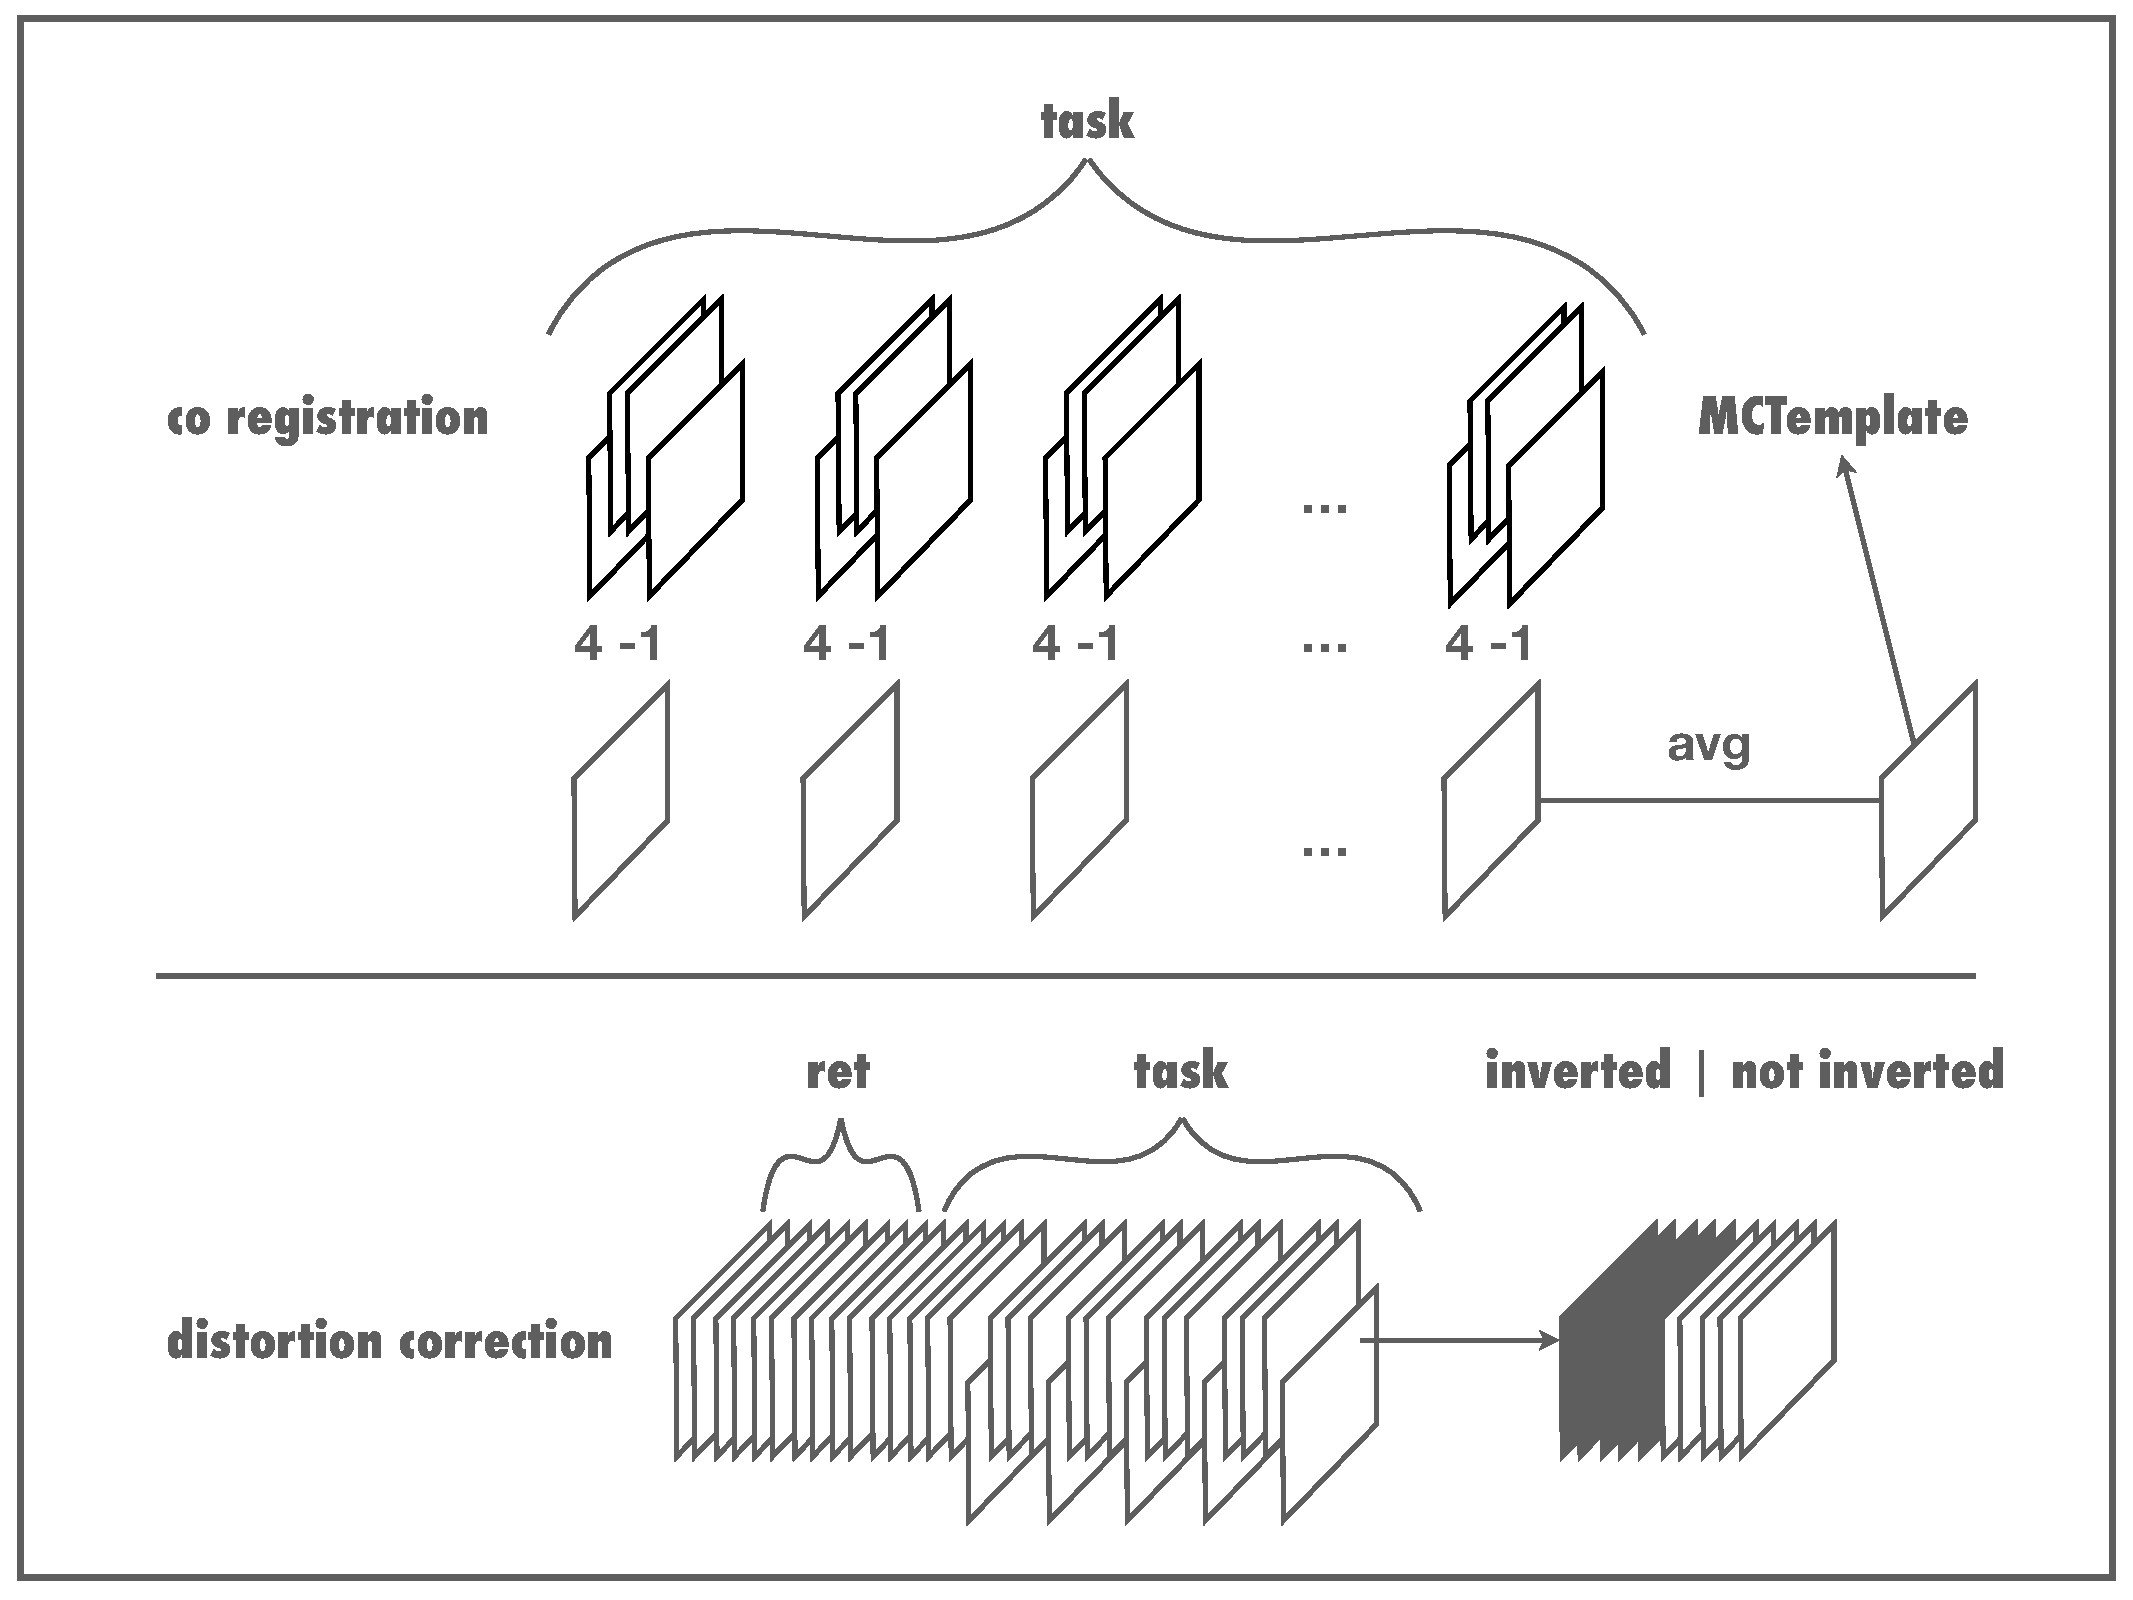
\includegraphics[width=0.8\textwidth]{coregdist}
\caption[Coregistration and distortion correction visual depiction]{Coregistration and distortion correction visual depiction}
\label{fig:coregdist}
\end{center}
\end{figure}

\subsection{pRF mapping}
Population receptive field mapping. Estimates retinotopic mapping from screen to cortical locations. This is to be done in order to obtain boundaries for visual areas such as V1, V2 and V3. First the fMRI time series will be interpolated (cubic) to match the numeber of frames presented during the stimulation. Afterwards pRF mapping will be analyzed and paramters will be written to volume files (NiFTI) and surface files for use with FreeSurfer.
\begin{table}[h]
%\centering
\begin{tabular}{l | r}
\toprule
maximum memory required & approx time required\\\toprule
64GB (480GB) & $\approx 8h$ \\\bottomrule
\end{tabular}
\end{table}
\FloatBarrier
\noindent Interpolate time series of volumes to match the number of presented frames during stimulation, by resampling the TR to match the "stimulation-frame-rate". The function below calls submits the corresponding MATLAB script as a qsub job.\\
The data will furthermore be transformed into percent change relative to the mean.\\

\noindent Results can be found in 4\_retinotopy/\\
\begin{lstlisting}[
    language=Shell,
    basicstyle=\ttfamily,
    breaklines=true]
    # interpolate volume time series
    sh do_tseriesinterpolation.sh
\end{lstlisting}
Once the data is in the right space to estimate voxel activity, based on active screen pixels, population receptive field mapping can be performed. Since using high resolution fMRI leads inevitably to "big data" the analysis has to be split up into multiple parts. In the present case an assumed computation time of $\approx 8h$ is reached by splitting up the analysis into 80 parts. Hence there is a linear relationship between processing time and parts the data can be split up to. In the present case all together $480~GB$ of memory are used to perform the analysis in parallel on 80 different cluster nodes with only $6~GB$ each. Afterwards results are combined into a single results file and temporary results are deleted.\\

\noindent Results can be found in 4\_retinotopy/\\
\begin{lstlisting}[
    language=Shell,
    basicstyle=\ttfamily,
    breaklines=true]
    # perform pRF mapping by splitting up the search space of voxels and combining the results.
    sh do_split_analyzePRF.sh
    sh combine_split_PRF_results.sh
\end{lstlisting}
After for each voxel certain parameters like circular coordinates mapping to screen locations, those have to be transformed into voluems, that can be overlayed with anatomical data in order to define masks for regions of interest based on the pRF mapping.\\

\noindent Results can be found in 4\_retinotopy/\\
\begin{lstlisting}[
    language=Shell,
    basicstyle=\ttfamily,
    breaklines=true]
    # transform pRF mapping results into NifTI volume overlays
    sh make_PRF_overlays.sh
    sh runonqsub.sh 16gb makeOverlays.sh
\end{lstlisting}
The retinotopy can also be performed in a single step, by calling the pipeline script:
\begin{lstlisting}[
    language=Shell,
    basicstyle=\ttfamily,
    breaklines=true]
    # using pipeline
    sh retinotopy.sh
\end{lstlisting}

\subsection{fMRI layer segmentation}
Gray matter boundaries will be used to compute cortical layer separation. First tksurfer is used to "draw" occipital ROIs based on the retinotopic mapping. Those regions will be transformed into gray matter masks such that an individual masks for V1, V2, V3 for each hemisphere exists. Cortical layer separation yields a probability map for each voxel to lay within a specifcially spaced area between gray matter boundaries. Thus a layer specific ROI specific map is created for each ROI by multiplying the ROI map with each of the layer probability maps. The results are 4D mask volumes separating the layer probabilies in the 4th dimension.
\begin{table}[h]
%\centering
\begin{tabular}{l | r}
\toprule
maximum memory required & approx time required\\\toprule
16GB & $\approx 0.5h+user$ \\\bottomrule
\end{tabular}
\end{table}
\FloatBarrier
FreeSurfer's tksurfer (\href{https://surfer.nmr.mgh.harvard.edu/fswiki/TkSurfer}{\nolinkurl{https://surfer.nmr.mgh.harvard.edu/fswiki/TkSurfer}}) is used to obtained visual ROIs from retinotopic mapping. When running GUI2ROIs.sh, an instance of tksurfer is spawned with the correct overlay already set up. In some cases the required file =0\_freesurfer/mri/orig.mgz is not present, but instead it's called orig\_nu.mgz. In that case please make sure that 0\_freesurfer/mri/orig.mgz exists by copy-pasting orig\_nu.mgz to orig.mgz\\
Afterwards run the commands below again. Once the overlay is displayed correctly, proceed as described in Section~\ref{sec:GUIprf}. Afterwards labels are transformed into masks. Since the selection was done on a surface, the corresponding mask volume is only one voxel thick. Hence voxel have to be expanded to fill the gray matter area.\\

\noindent Results can be found in 5\_laminar/\\
\begin{lstlisting}[
    language=Shell,
    basicstyle=\ttfamily,
    breaklines=true]
    # making masks for V1,2,3 based on retinotopy
    sh GUI2ROIs.sh
    sh labels2masks.sh
    sh expandROIs.sh
\end{lstlisting}
\begin{figure}
\begin{center}
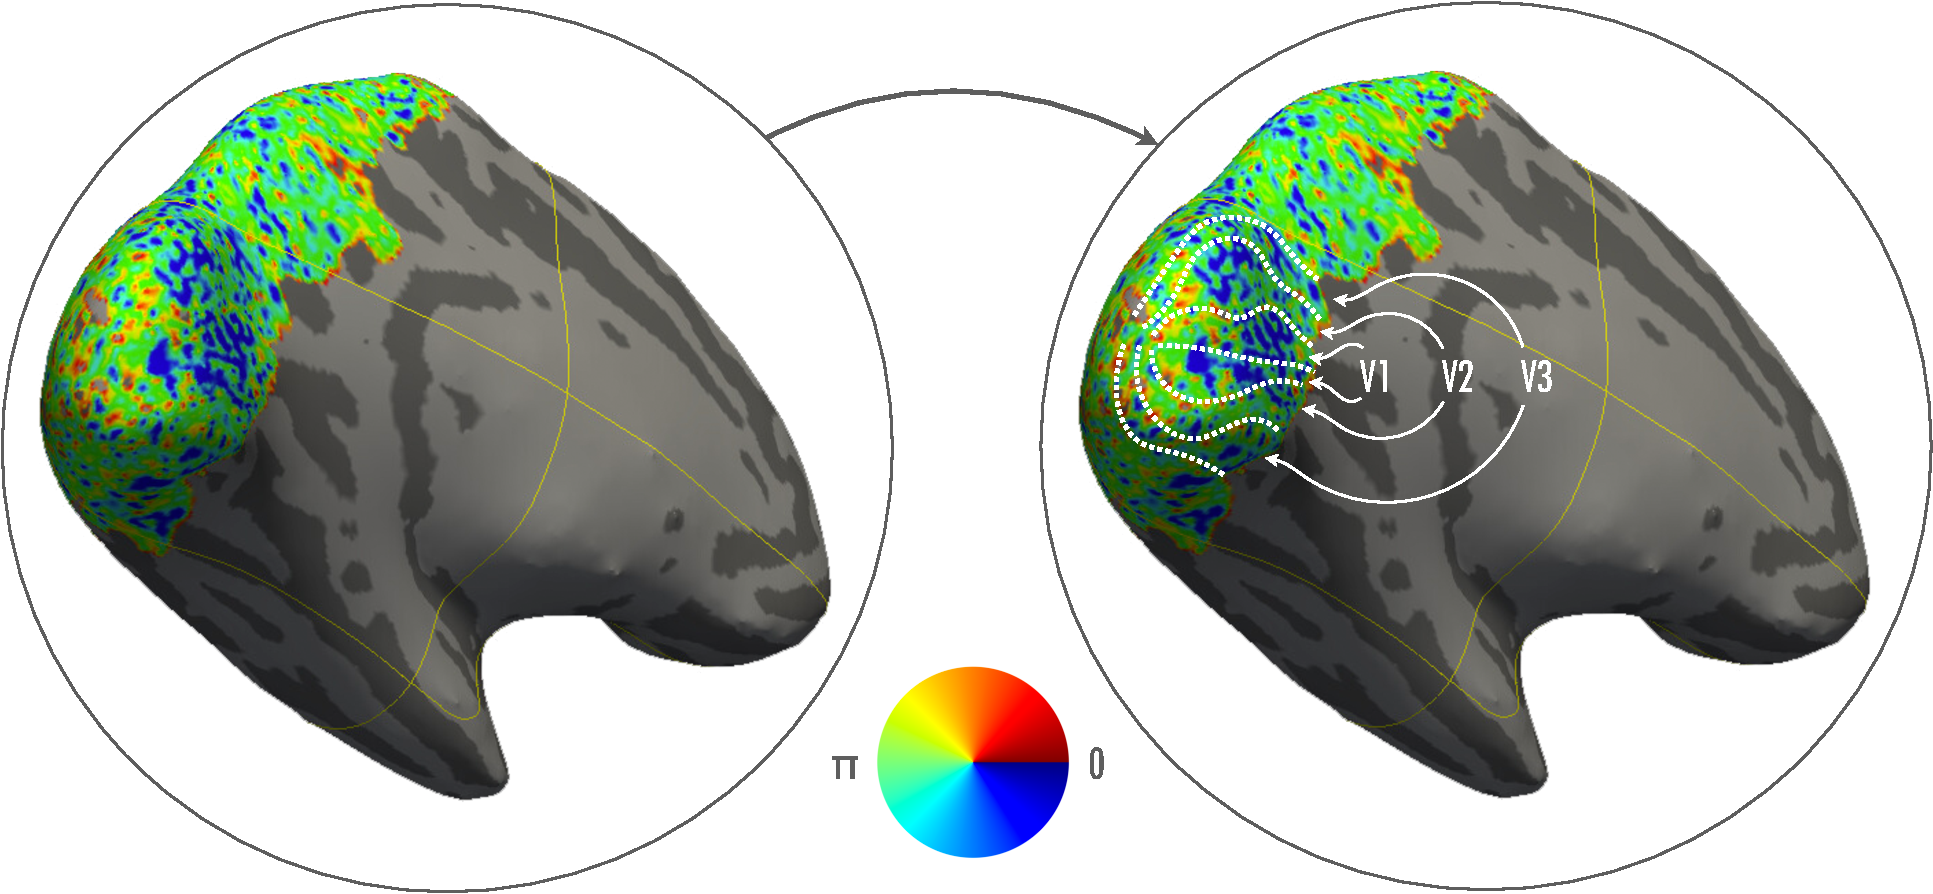
\includegraphics[width=1\textwidth]{ROIselpRF}
\caption[Example for visual ROI definition]{Definition of visual ROIs. Note that along the borders of visual areas a significant shift in color occurs.}
\label{fig:ROIpRF}
\end{center}
\end{figure}
Note that using FreeSurfer's freeview yields better plotting functionality, however TkSurfer provides an easier way to select vertices.\\
Once this is done gray matter volumes are split into corical layers. This is implemented in OpenFmriAnalysis (\href{https://github.com/TimVanMourik/OpenFmriAnalysis}{\nolinkurl{https://github.com/TimVanMourik/OpenFmriAnalysis}}). Based on gray and white matter boundaries and the respective curvature, gray matter is segmented into 3 layers. The result is a probability map for each voxel to belong to a certain layer.\\

\noindent Results can be found in 5\_laminar/\\
\begin{lstlisting}[
    language=Shell,
    basicstyle=\ttfamily,
    breaklines=true]
    # performing laminar separation
    sh do_getLayers.sh
    sh do_getLayerWeights.sh
\end{lstlisting}
The layer segmentation process can also be performed in a single step, by calling the pipeline script:
\begin{lstlisting}[
    language=Shell,
    basicstyle=\ttfamily,
    breaklines=true]
    # using pipeline
    sh laminar.sh
\end{lstlisting}
\FloatBarrier
\subsection{EEG pre-processing}
The raw EEG signal will be transformed into virtual channel data by applying a LCMV beamformer. Frequencies of interest ($\alpha$, $\beta$, $\gamma$) are defined that $8~Hz \leq \alpha \leq 12~Hz$; $18~Hz \leq \beta \leq 28~Hz$; $60~Hz \leq \gamma \leq 80~Hz$. Since the covariance matrices of the noise will differ significantly for lower and higher frequencies, the data will be band pass filtered for low and high frequencies separately. This will be achieved by using pass bands of $2-32~Hz$ and $30-100~Hz$ respectively.\\
A FEM forward model will be used as well as a anatomical constraint source model (see Figure~\ref{fig:exampleSourcemodel} for a graphical depiction).\\
\begin{table}[h]
%\centering
\begin{tabular}{l | r}
\toprule
maximum memory required & approx time required\\\toprule
$16~GB$ & $\approx 2h$ \\\bottomrule
\end{tabular}
\end{table}
First data is loaded an segmented into trials. Note that the default trial selection string might vary from experiment to experiment. Target trigger values can be set in do\_EEGpreprocessing.sh\\
Additionally the data will be band pass filtered at $2-32~Hz$ for $\alpha$ and $\beta$ bands and at $30-100~Hz$ for $\gamma$. Respective changes in the filterband can be made in do\_EEGpreprocessing.sh\\
If desired, trials should be excluded at this stange as well. To achieve this either use FieldTrip's built in functionality (do\_EEGpreprocessing.sh bottom) or provide a logical array of whether to include a trial to ft\_redefinetrial(cfg, data). See \href{http://www.fieldtriptoolbox.org/reference/ft_redefinetrial}{\nolinkurl{http://www.fieldtriptoolbox.org/reference/ft\_redefinetrial}} for more information.\\

\noindent Results can be found in 6\_EEG/\\
\begin{lstlisting}[
    language=Shell,
    basicstyle=\ttfamily,
    breaklines=true]
    # EEG preprocessing: trial selection, BP filter, (trial selection)
    sh do_EEGpreprocessing.sh
\end{lstlisting}
Once the general preprocessing is done, the function ft\_timelockanalysis (\href{http://www.fieldtriptoolbox.org/reference/ft\_timelockanalysis}{\nolinkurl{http://www.fieldtriptoolbox.org/reference/ft\_timelockanalysis}}) is used to estimate the noise covariance matrix based on baseline data for high and low frequencies separately. This is necessary since the noise structure for those different bands varies significantly. The default noise estimation window is $-0.5$ to $-0.1~s$ realtive to stimulus onset.\\

\noindent Results can be found in 6\_EEG/\\
\begin{lstlisting}[
    language=Shell,
    basicstyle=\ttfamily,
    breaklines=true]
    # EEG preprocessing: noise estimation
    sh do_EEGtimelock.sh
\end{lstlisting}
As last step the result from fsrecon (do\_fsrecon.sh) must be prepared to be used as source model. For this purpose Workbench (\href{https://github.com/Washington-University/workbench}{\nolinkurl{https://github.com/Washington-University/workbench}}) is used, wrapped into do\_EEGprepareFS.sh\\

\noindent Results can be found in 6\_EEG/\\
\begin{lstlisting}[
    language=Shell,
    basicstyle=\ttfamily,
    breaklines=true]
    # EEG preprocessing: source model preparation
    sh do_EEGprepareFS.sh
\end{lstlisting}


\subsection{EEG prepare head and source models}
Head and Sourcemodel are prepared using FieldTrip. Per default the pipeline is set up to use finite element models (FEM), but can be changed to boundary element model (BEM) as well. As source model, the result from Workbench is used.
\label{sec:Sourcemodel}
\begin{table}[h]
%\centering
\begin{tabular}{l | r}
\toprule
maximum memory required & approx time required\\\toprule
$32~GB$ & $\approx 6h+user$ \\\bottomrule
\end{tabular}
\end{table}
Loading and segmenting anatomical MRI data is done using ft\_volumesegment (\href{http://www.fieldtriptoolbox.org/reference/ft\_volumesegment}{\nolinkurl{http://www.fieldtriptoolbox.org/reference/ft\_volumesegment}}) and ft\_prepare\_mesh (\href{http://www.fieldtriptoolbox.org/reference/ft\_prepare\_mesh}{\nolinkurl{http://www.fieldtriptoolbox.org/reference/ft\_prepare\_mesh}}). For more details about the settings of this function see Section~\ref{sec:prepHM}.\\

\noindent Results can be found in 6\_EEG/\\
\begin{lstlisting}[
    language=Shell,
    basicstyle=\ttfamily,
    breaklines=true]
    # prepare head model
    sh do_EEGprepareHeadmodel.sh
\end{lstlisting}
Once the headmodel is prepare, sensor locations need to be coregistered. This is achieved by starting an interactive MATLAB session and opening the script B\_scripts/\textbf{do\_EEGelectrodeRegistration.m}. The FieldTrip function ft\_electroderealign is used to interactively coregister sensor locations to anatomical MR data. See \href{http://www.fieldtriptoolbox.org/reference/ft\_electroderealign}{\nolinkurl{http://www.fieldtriptoolbox.org/reference/ft\_electroderealign}} for more information.\\

\noindent Results can be found in 6\_EEG/\\
\begin{lstlisting}[
    language=Shell,
    basicstyle=\ttfamily,
    breaklines=true]
    # coregister electrode locations to anatomical MR using MATLAB
    matlab
\end{lstlisting}
The previously computed data is now prepared to be finally used and the Workbench sourcemodel is loaded.\\

\noindent Results can be found in 6\_EEG/\\
\begin{lstlisting}[
    language=Shell,
    basicstyle=\ttfamily,
    breaklines=true]
    # prepare data and load source model
    sh do_EEGprepareSourcemodel.sh
\end{lstlisting}
\begin{figure}
\begin{center}
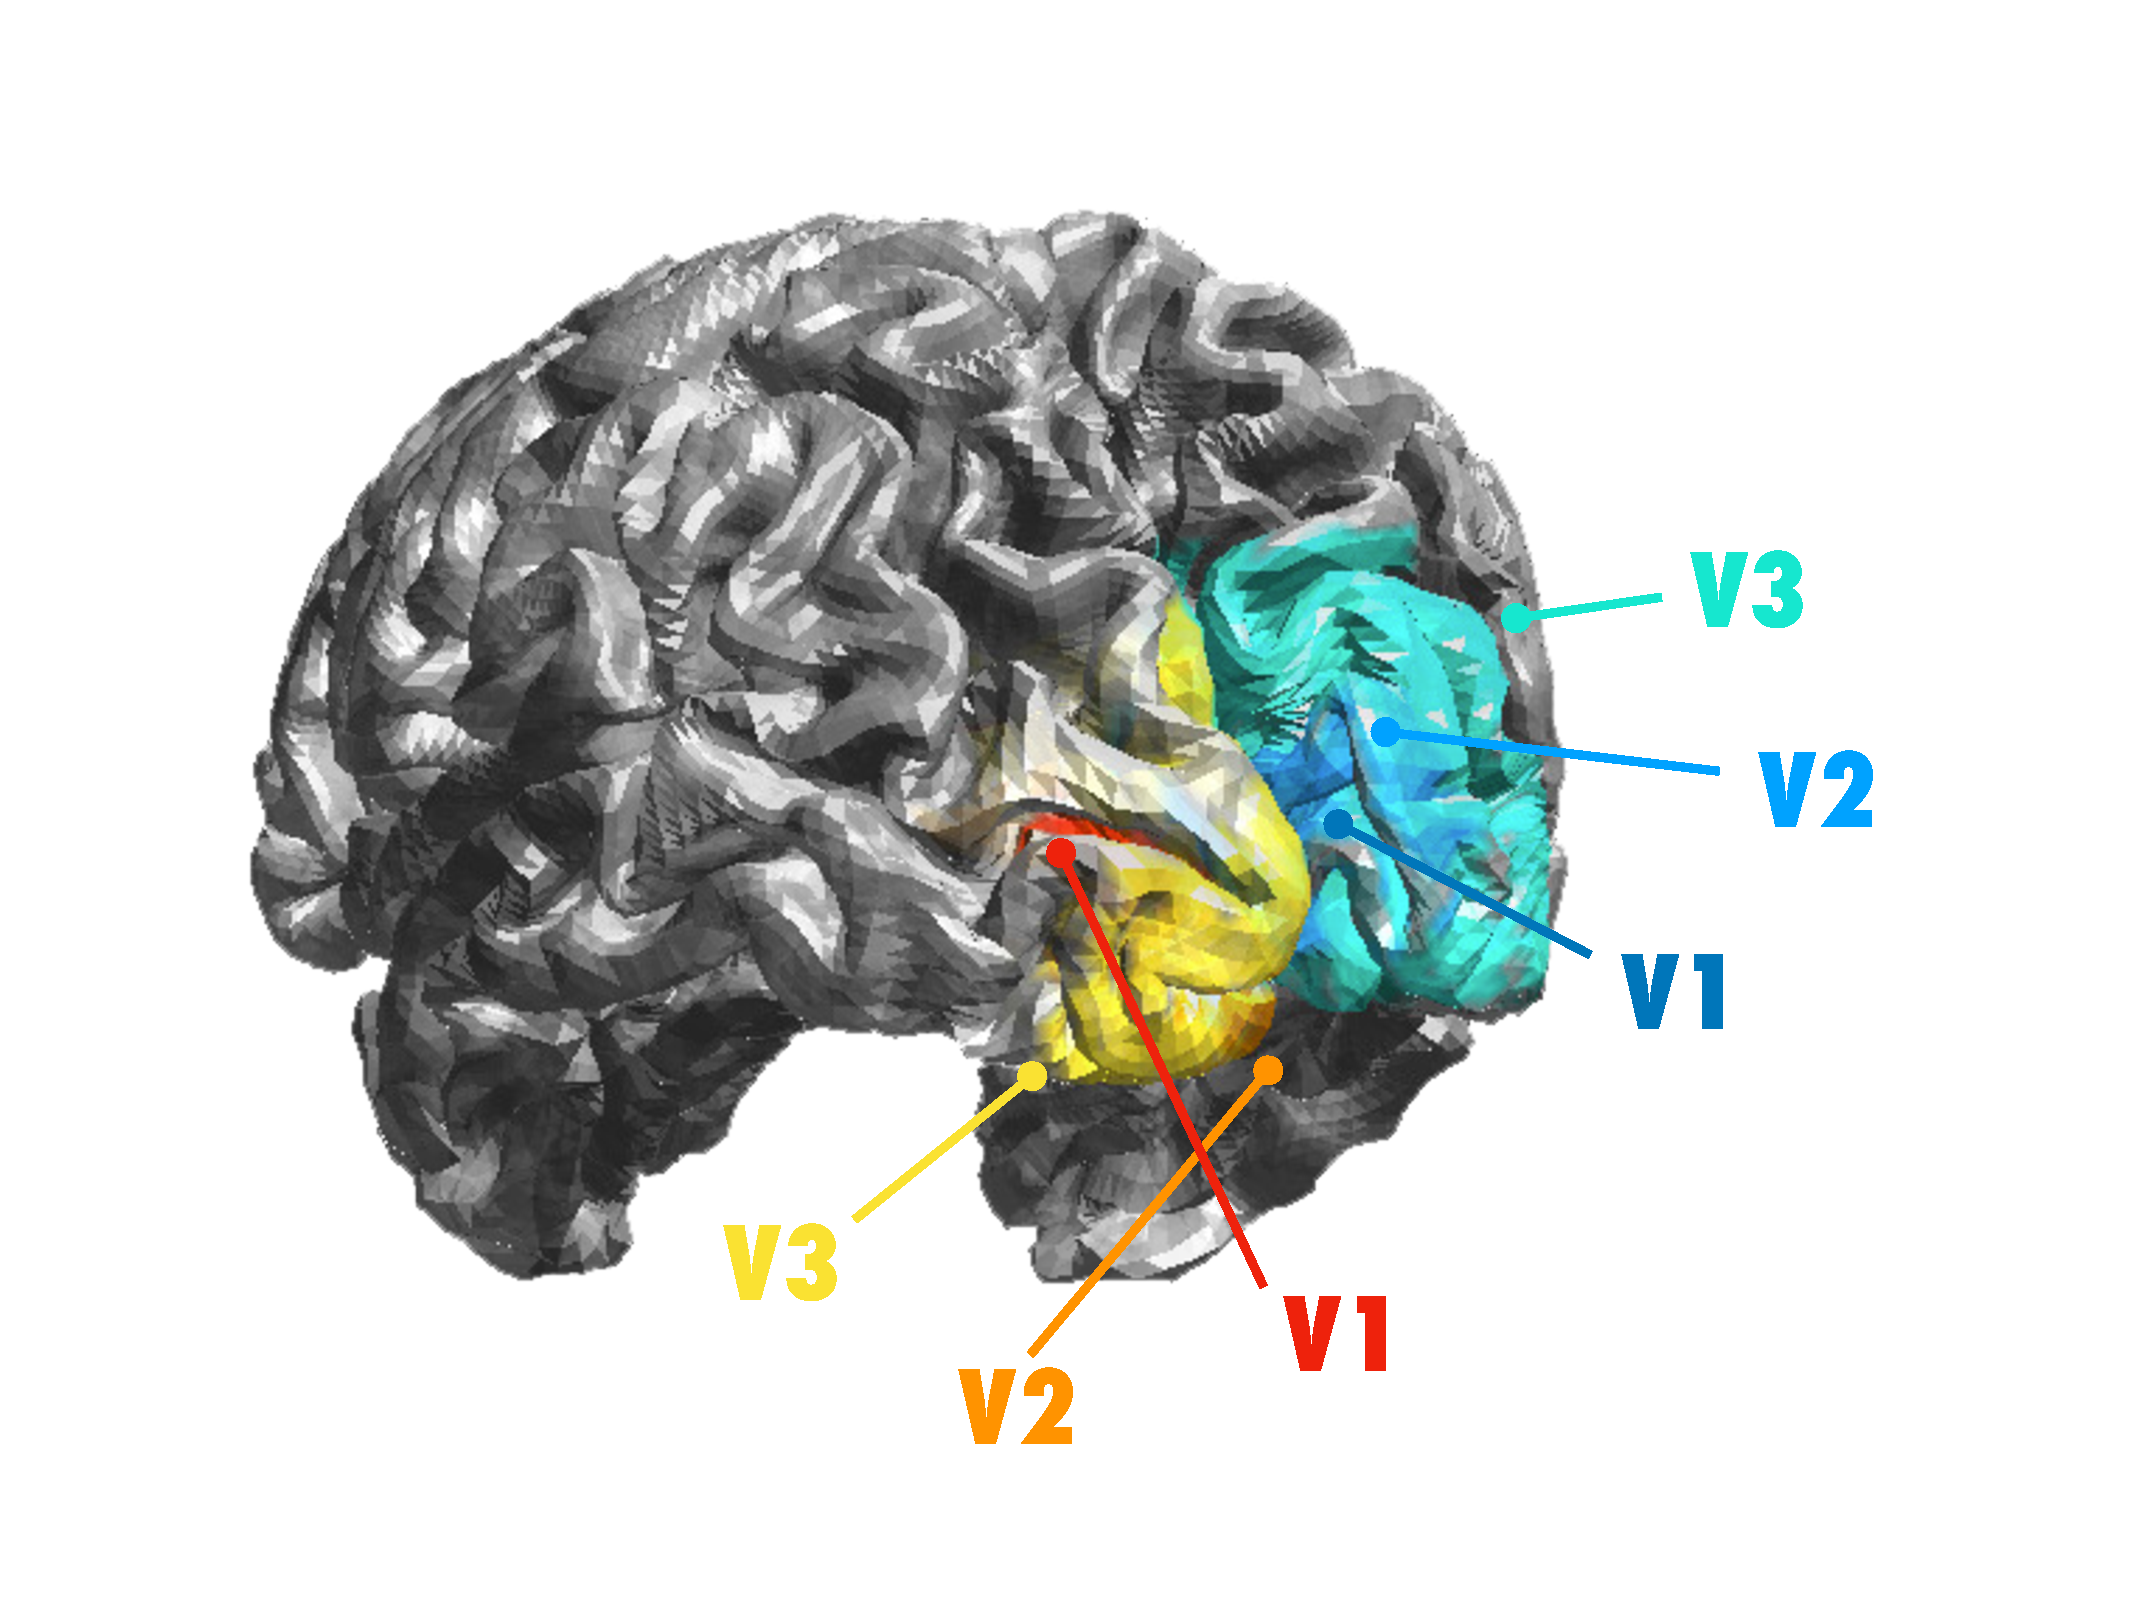
\includegraphics[width=0.8\textwidth]{exampleSourcemodel}
\caption[Example source model]{Example source model including visual ROIs. Note that for demonstrative purposes all possible ROIs are show, however per default only V1 for both hemispheres will be used. This plot was created using EEGvisualizeVirtualChannel.m}
\label{fig:exampleSourcemodel}
\end{center}
\end{figure}
\FloatBarrier
\subsection{EEG compute virtual channels}

\begin{table}[h]
%\centering
\begin{tabular}{l | r}
\toprule
maximum memory required & approx time required\\\toprule
$960~GB$ & $\approx 12h$ \\\bottomrule
\end{tabular}
\end{table}
The first step is to estimate time courses for dipoles at each voxel lcoation. To achieve this LCMV beamformer weights are computed separately for high and low frequencies. To reduce search space and hence computation time, previously computed ROI maps are used. By default left and right V1 are used as two separate ROIs. Volumetric ROIs are translated into cartesian coordinates. Beamformer weights are computed using $\lambda=10\%$ for noise regularization employing ft\_sourceanalysis (\href{http://www.fieldtriptoolbox.org/reference/ft\_sourceanalysis}{\nolinkurl{http://www.fieldtriptoolbox.org/reference/ft\_sourceanalysis}}). Trial segmented data is then multiplied with beamformer weights, in order to obtain individual time series for all dipole locations.\\
Note that $480~GB$ of memory are required to estimate the beamformer weights in a parallelized fashion as below.\\

\noindent Results can be found in 6\_EEG/\\
\begin{lstlisting}[
    language=Shell,
    basicstyle=\ttfamily,
    breaklines=true]
    # prepare data and load source model
    sh do_EEGsplitBeamformer.sh
    sh do_EEGsplitVirtualChannel.sh
\end{lstlisting}
Afterwards a time frequency analysis (\href{http://www.fieldtriptoolbox.org/reference/ft\_freqanalysis}{\nolinkurl{http://www.fieldtriptoolbox.org/reference/ft\_freqanalysis}}) is run for all virtual channels. Since this operation is performed on a single trial basis for different filter bands and left and right hemisphere separately, $960~GB$ of memory are required to compute this step as implemented.\\

\noindent Results can be found in 6\_EEG/\\
\begin{lstlisting}[
    language=Shell,
    basicstyle=\ttfamily,
    breaklines=true]
    # prepare data and load source model
    sh do_EEGsplitFreqOnVirtChan.sh
\end{lstlisting}
To relate the data to layer specific fMRI results, a channel selection has to take place, that is optimized for frequency ROIs ($\alpha, \beta, \gamma$). For each of the 3 bands all virtual channels will be searched and the best 100 are selected. Those are defined to have the lowest ($\alpha, \beta$) or highest ($\gamma$) relative power compared to the baseline period ($-0.3$ to $-0.2~s$ relative to simulus onset).\\

\noindent Frequency ROIs are defined as:
\begin{table}[h]
%\centering
\begin{tabular}{c | c | c}
\toprule
$\alpha$ & $\beta$ & $\gamma$\\\toprule
$8-12~Hz$ & $22-28~Hz$ & $50-70~Hz$ \\\bottomrule
\end{tabular}
\end{table}\\
Furthermore, the function produces figures saved in C\_miscResults similar to what is shown in Figure~\ref{fig:exampleGamma}.\\

\noindent Results can be found in 6\_EEG/\\
\begin{lstlisting}[
    language=Shell,
    basicstyle=\ttfamily,
    breaklines=true]
    # prepare data and load source model
    sh do_EEGfreqChanSelect.sh
\end{lstlisting}
\begin{figure}
\begin{center}
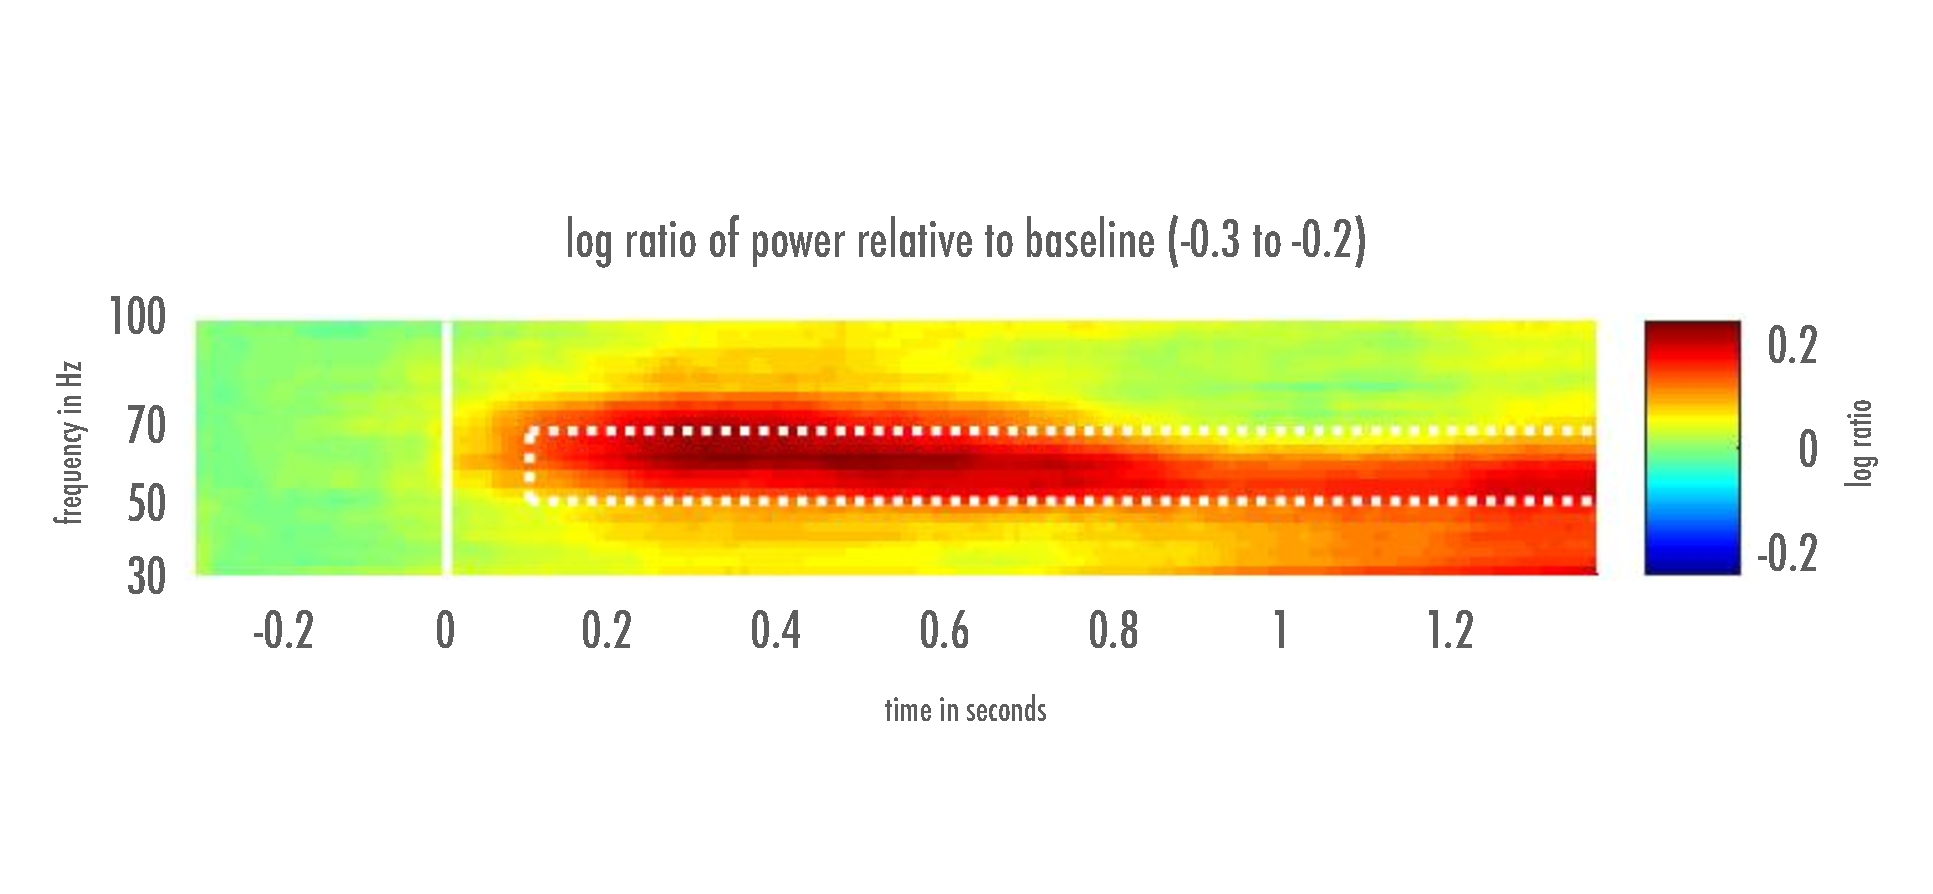
\includegraphics[width=1\textwidth]{exampleGamma}
\caption[Example for $\gamma$ response in virtual channel]{Example for $\gamma$ response in virtual channel}
\label{fig:exampleGamma}
\end{center}
\end{figure}
\FloatBarrier

\section{Scripts explained (support for runonqsub.sh: Q)}
\subsection{getToolboxes.sh}
\label{sec:getTools}
Downloads all necessary toolboxes into a folder called toolboxes/ or displays a URL where the user has to download the software manually (see Section~\ref{sec:prereq}). That is FSL and SPM have to be downloaded manually due to required user registration. Place them in the same directory as the other toolboxes or install as required.

\subsection{runonqsub.sh}
Initiates a qsub session and sends it to the cluster. This is necessary, since scripts running on the cluster are copied to a different directory, but within scripts all directories are relative. runonqsub.sh must hence be run in a "normal" session not using a non-interactive qsub, giving the respective script that was intended to run as an argument. runonqsub will then set everything up correctly. Further you have to specify the amount of memory needed.
\begin{lstlisting}[
    language=Shell,
    basicstyle=\ttfamily,
    breaklines=true]
    # example
    sh runonqsub.sh 32gb myscript.sh
\end{lstlisting}

\noindent Additional arguments can be passed after the script.\\
\begin{lstlisting}[
    language=Shell,
    basicstyle=\ttfamily,
    breaklines=true]
    # example with argument
    sh runonqsub.sh 32gb myscript.sh myargument
\end{lstlisting}
\noindent Under the hood:
\begin{itemize}
\item a qsub session is initiated like so: qsub -l walltime=24:00:00,mem=\$1 -F "\$DIR \$\{@:3\}" \$DIR/\$2
\item \$DIR is the current absolute path to B\_scripts
\item \$1 is the amount of memory used (e.g. 32gb)
\item \$2 is the respective script to run (e.g. myscript.sh)
\item \$\{@:3\} is all following arguments that are parsed to the script
\item every time runonqsub.sh is called the absolute path is forwarded to the script (-F \$DIR) in order to keep the relative dependencies clear
\end{itemize}

\subsection{cleanscriptsfolder.sh}
Since qsub puts a output + error log into /B\_ scripts cleanscriptsfolder.sh can be used to move all qsub outputs to /B\_scripts/qsuboutput\\

\subsection{liveupdateqsub.sh}
Submits a qstat -u user request every second.
\begin{lstlisting}[
    language=Shell,
    basicstyle=\ttfamily,
    breaklines=true]
    # example
    sh liveupdateqsub.sh tomcla
\end{lstlisting}

\noindent exit command by hitting ctrl+c

\subsection{waitForJobs.sh}
Checks all currently running jobs (qstat -u user) and waits until the last script up until this point has finished.

\subsection{makenewsubject.sh}
executable script (double click to execute)\\

Creates a new subject (S\#) folder structure in order to get all folder dependencies right. It automatically detects folders called "S\textit{number}" and creates a new folder incrementing \textit{number} by one.

\subsection{setupfolders.sh (Q)}
Sets up the necessary folder structure for the analysis (within a subject folder). This function is automatically called when using makenewsubject.sh\\

\subsection{do\_preparefunctionals.sh (Q)}
\label{sec:prepfct}
Prepares functional data, i.e. removes the first 4 and the last x volumes of every set of functionals, where x is the number of volumes acquired after the stimulation ended. If files were modified (i.e. if volumes were deleted), the original file will remain in /niftis/functionals/old\\

\subsection{do\_realignment.sh (Q)}
\label{sec:realign}
Merges and motion corrects all files in /niftis/functionals using the average volume of all task volumes.\\

\noindent numberofvolumes.txt is written to /A\_helperfiles giving information about which sets had how many volumes. The first column is coresponds to dim4 from fslinfo\\

\noindent Under the hood:
\begin{itemize}
\item fslmerge is called to create a combined .nii for all files in niftis/functionals/*sparse* - files are merged allong the 4th dimension
\item a .txt file is created saving which files were merged and how many volumes were in there
\item mcflirt is used on the combined data doing the motion correction based on the average volume across all task blocks
\item all results are stored in /1\_realignment
\item results have the extension "\_mcf"
\end{itemize}

\subsection{do\_distcorr.sh (Q)}
\label{sec:distcorr}
Uses the averge volume of the inverted set of images in /niftis/inverted as reference for \textit{inverted}\\

\noindent Uses as many volumes \textit{n} as there were in /niftis/inverted. Respective volumes are selected starting from the last going in \textit{4 x n} steps backward. Hence the resulting average of this set was computed over the 4th volume of each of \textit{n} last sets in the normal images. Simplified (all 1 are selected):\\

\noindent for n=5\\

\noindent 0,0,0,0,...,0,0,0,1,0,0,0,1,0,0,0,1,0,0,0,1,0,0,0,1\\

\noindent Both (normalavg and invertedavg) will be used to esimate the distortion correction.\\

\noindent Under the hood:
\begin{itemize}
\item reference volumes (normal + inverted) are selected in order to do the field distortion estimate (selection: see above).
\item selected reference volumes are merged into a single file (/3\_distcorrection/all\_b0.nii.gz)
\item topup is called using the merged (normal + inverted) .nii and performs field mapping accoriding to the specifications in /A\_helperfiles/b02b0.cnf using the acquisition parameters specified in acquisition\_parameters.txt
\item all results are stored in /3\_distcorrection
\end{itemize}

\subsection{do\_applysimpledistcorr.sh (Q)}
\label{sec:applydistcorr}
Applies distortion correction to all functional data.\\

\noindent Under the hood:
\begin{itemize}
\item distortion correction is applied to the full set of functionals using the OUTPUT of topup (topup [$\ldots$] --out=OUTPUT) as well as acquisition\_parameters.txt (Using --method=jac)
\item all results are stored in /3\_distcorrection
\item all results have the prefix "corrected\_"
\end{itemize}

\subsection{do\_preparecoregistration.sh (Q)}
\label{sec:prepcoreg}
Computes a reference volume (MCTemplate) used as the basis  to co-register with the anatomical image. This image is computed by splitting the entire set of task volumes into chunks of 4. In each chunk the 1st volume is substracted from the 4th. This procedure yields a pseude-T1 contrast. All chunk differences are then averaged to form "MCTemplate"

\subsection{do\_correctavgdiff.sh (Q)}
\label{sec:corravg}
Due to the subtraction of the 1st from the 4th volume the area outside the brain has the highest value. In order to correct this the lowest value will be shifted to zero the a certain part of the higher values are cut (e.g. 0.975).\\

\noindent The result should be checked using "fsleyes ../2\_coregistration/Inplane/MCTemplateThr*.nii.gz" to ensure that the area outside the brain is nulled. Note that it can happen that some areas within the brain are nulled as well. If they are not too wide spread they do not affect later co-registration.

\subsection{do\_fsrecon.sh (Q)}
\label{sec:fsrecon}
Performs segmentation using Freesurfer.\\

\noindent If running on OSX the script assumes:
\begin{lstlisting}[
    language=Shell,
    basicstyle=\ttfamily,
    breaklines=true]
    # FreeSurfer Home Mac
    FREESURFER_HOME=/Applications/freesurfer
\end{lstlisting}

\noindent If running on linux the script assumes:\\
\begin{lstlisting}[
    language=Shell,
    basicstyle=\ttfamily,
    breaklines=true]
    # FreeSurfer Home Linux
    FREESURFER_HOME=/opt/freesurfer/version
\end{lstlisting}

\noindent The target image that is used for the segmentation must be located in /niftis/t1\\

\noindent Under the hood:
\begin{itemize}
\item calls recon-all -i /niftis/t1/* -subjid  0\_freesurfer -all
\item all results are stored in /0\_freesurfer
\end{itemize}

\subsection{do\_coregistration.sh}
\label{sec:coreg}
Will submit a qsub session using MATLAB, that in turn will be using FreeSurfer (bbregister) and OpenFmriAnalysis to perform a linear and non-linear boundary registration.  Movie files of the respective co-registration are stored in /C\_miscResults

\noindent The file used to execute MATLAB commands is /B\_scripts/do\_coregistration.m Note that it will be modified using the correct folder settings, which yields tmp.m that will be called and removed after MATLAB was closed.\\

\subsection{do\_coregistration.m}
The script doing the actual co-registration. Uses wrapper functions from OpenFmriAnalysis to evoke FreeSurfers bbregister and computes a recursive boundary based registration.\\

\noindent The results are seevral files storing the boundaries as a point cloud, and the respective transformation in diferent formats.

\noindent Under the hood:
\begin{itemize}
\item calls bbregister
\item results are stored in /2\_coregistration
\item yields boundaries.mat, matrix.mat, bbregister.dat, transmat.txt, transmatinv.txt
\end{itemize}

\subsection{do\_makemasksandlabels.sh (Q)}
\label{sec:msklbl}
example: sh do\_makemasksandlabels.sh\\

\noindent Uses FreeSurfer reconstruction to create masks for CSF, gray matter and white matter and creates labeled volume for use within retinotopy containing left / right + gray / white matter. All masks will be created as full-brain and partial-brain masks.\\

\noindent If the orientation needs to be changed, parse the respective FreeSurfer compatible orientation parameter (\href{https://surfer.nmr.mgh.harvard.edu/pub/docs/html/mri_convert.help.xml.html}{\nolinkurl{https://surfer.nmr.mgh.harvard.edu/pub/docs/html/mri\_convert.help.xml.html}})\\

\noindent Under the hood:
\begin{itemize}
\item moves anatomical volumes to functional space calling do\_movesinglevolume.sh InputVolume.nii.gz transmat.txt OutputVolume.nii.gz
\item results are stored in /2\_coregistration
\item coregistered functional masks have the prefix "fct" and the suffix "coreg"
\end{itemize}

\subsection{do\_movesinglevolume.sh}
Simple wrapper function to apply a transformation from one volumetric space to another, given a transformation matrix.\\

\noindent Under the hood:
\begin{itemize}
\item flirt -applyxfm -in \$1 -ref \$1 -init \$2 -out \$3
\item \$1: volume to move
\item \$2: transformation matrix in form of a .txt file containing a $4\times4$ transformation matrix
\end{itemize}

\subsection{do\_tseriesinterpolation.sh}
\label{sec:tseriesinterp}
Wrapper function for do\_tseriesinterpolation.m Variables used by do\_tseriesinterpolation.m can be defined in the header section of the script.

\noindent Under the hood:
\begin{itemize}
\item submits a MATLAB job using qsub calling do\_tseriesinterpolation.m using the below settings
\item default number of blocks: 3
\item default TR: 2.7s
\item default Mask Threshold: 0.01
\item default rescaled stimulus size: 100px
\end{itemize}

\subsection{do\_tseriesinterpolation.m}
Interpolates time series for retinotopy scans to match the number of frames during the stimulation (cubic interpolation). The new TR will be $TR_{new}=\frac{TR_{old}N_{volumes}}{N_{imageframes}}$. The function implements "tseriesinterp" from the analyzePRF toolboxe. The data will be normalized to percent signal change.\\

\noindent Furthermore all images will be downsampled to the predefined size (e.g. 100px)\\

\noindent Under the hood:
\begin{itemize}
\item interpolates time series of functional data to match the numer of frames during the stimulation
\item results: tIntData.mat (interpolated time series)
\item results: mask.mat (volume mask)
\item results: voxelindices.mat (indices of mask voxels, ratio between $N_{imageframes}$ and $N_{volumes}$, mask threshold)
\item results: downsampled images
\end{itemize}

\subsection{do\_split\_analyzePRF.sh}
\label{sec:splitanalyzePRF.sh}
Wrapper function to call do\_analyzePRF.sh The function calls a predefined number of instances of do\_analyzePRF.sh to run on the cluster, submitted using qsub. Per default 80~jobs requesting 6~GB of memory each (see Section~\ref{sec:analyzePRF.sh}), will be spawned. This procedure speeds up the population receptive field estimation significantly and would be otherwise impractical on high resolution functional data.\\

\subsection{do\_analyzePRF.sh}
\label{sec:analyzePRF.sh}
Wrapper function to call do\_analyzePRF.m Spawns a qsub job using 6GB of memory (default) and runs a specific part of a set of parts. The first input argument is the part that is to be computed and the second input argument is the sum of all parts.
\begin{lstlisting}[
    language=Shell,
    basicstyle=\ttfamily,
    breaklines=true]
    # example split search space into 5 parts an run the first
    sh do_analyzePRF.sh 1 5
\end{lstlisting}
\begin{lstlisting}[
    language=Shell,
    basicstyle=\ttfamily,
    breaklines=true]
    # example not splitting up search space
    sh do_analyzePRF.sh 1 1
\end{lstlisting}

\subsection{do\_analyzePRF.m}
Computes pRF mapping implemeting "analyzePRF" from the analyzePRF toolbox. It can be decided whether to average across blocks or if the estimates shall be done for each block separately and averaging the results. Note, that running the analysis on separate blocks slows down computation time, but to my experience yields slightly better results.\\

\noindent Under the hood:
\begin{itemize}
\item estimates pRFs
\item computes pRF mapping for part x of X by splitting the list of indices and selecting the corresponding set
\item set avgdata=1 to average data before the analysis (otherwise it will be averaged afterwards)
\item result: structure containing pRF parameters of part x of X
\end{itemize}

\subsection{combine\_split\_PRF\_results.sh}
\label{sec:combsplt}
Wrapper function for combine\_split\_PRF\_results.m Combines split results from do\_split\_analyzePRF.sh (see Section~\ref{sec:splitanalyzePRF.sh}). Note that the exact amount of parts that the data was split into must be defined here (default: 80).\\

\subsection{combine\_split\_PRF\_results.m}
Combines split results from do\_split\_analyzePRF.sh (see Section~\ref{sec:splitanalyzePRF.sh}) into a single MATLAB file. Note that given the respective numerical naming of all parts (x\_of\_X) parts will be concatenated along values of x. After this operation split parts will be deleted.

\subsection{make\_PRF\_overlays.sh}
\label{sec:mkprfO}
Wrapper function for make\_PRF\_overlays.m

\subsection{make\_PRF\_overlays.m}
Takes result of pRF mapping and creates .nii files for separate parameters (ang, ecc, expt, r2, rfsize, xpos, ypos). The data will be saved in ../4\_retinotopy as parameterName\_map.nii\\

\noindent Under the hood:
\begin{itemize}
\item angle ($\theta$) will be devided by 180 and multiplied by $\pi$
\item eccentricity ($r$) will be devided by the image size (in px) and multiplied by the original value range ($^\circ$ visual angle; default: 7). Only ecc values that have a positive $R^2$ and are smaller than the defined field of view, will be written to file. All other values will be set to $NaN$
\item X position (xpos) $\cos(\theta)\cdotp r$
\item Y position (ypos) $\sin(\theta)\cdotp r$
\end{itemize}

\subsection{makeOverlays.sh (Q)}
\label{sec:mkOver}
Makes FreeSurfer compatible overlays from NiFTI files. Calls FreeSurfer's "mri\_vol2surf" in order to transform a volumetric .nii file into a surface file. This will be done for both hemispheres separately. Parameters transformed to surface files are: ang, ecc, xpos, ypos, r2\\

\noindent Under the hood:
\begin{itemize}
\item mri\_vol2surf --src \$DIR/4\_retinotopy/ang\_map.nii  --srcreg \$DIR/2\_coregistration/bbregister.dat --hemi ?h --surf pial --out \$DIR/4\_retinotopy/?h.ang.mgh --out\_type paint
\item --src: NiFTI to be transformed
\item --srcreg: result from "bbregister" of do\_coregistration.sh (default: bbregister.dat)
\item --hemi: respective hemisphere (lh for left hemisphere or rh for right hemisphere)
\item --surf: surface used as reference (obtained from FreeSurfer in ../0\_freesurfer/surf/)
\item --out: output file name
\item --out\_type: influences how the file is outputted (see "mri\_vol2surf --help" for more information)
\end{itemize}

\subsection{GUI2ROIs.sh}
\label{sec:GUI2ROI}
This script spawns an instance for tksurfer (FreeSurfer)

\subsection{labels2masks.sh (Q)}
\label{sec:lbl2msk}

\subsection{expandROIs.sh}
\label{sec:expROI}

\subsection{expandROIs.m}

\subsection{tc\_expandVoxelSelection.m}

\subsection{do\_getLayers.sh}
\label{sec:getLyr}

\subsection{do\_getLayers.m}

\subsection{do\_getLayerWeights.sh}
\label{sec:getLyrW}

\subsection{do\_getLayerWeights.m}

\subsection{do\_EEGpreprocessing.sh}
\label{sec:EEGpreproc}
Wrapper function for running do\_EEGpreprocessing.m via qsub

\subsection{do\_EEGpreprocessing.m}
Does a basic preprocessing to the data. First trigger values will be extracted and trials are defined according to the specifications in the script. Further only EEG channels are selected. The Data is downsampled to $1024~Hz$. This in-between step is stored. Afterwards the data is further split into different sets of band pass filtered data. Note, that the noise structure will be different for high and low frequencies and thus this step is highly recommendable. Per default two band pass filters are chosen ($2-32~Hz$ and $30-100~Hz$). The baseline period will be from $-0.5~s$ until $-0.1~s$ relative to the stimulus onset. For the high frequency case a dft filter to filter line noise is applied. Using the default version of this function will store the computed data using the respective filter settings as a prefix. However if desired trials can / should be excluded in this step as well.\\

\noindent Under the hood (uses the following fieldtrip functions):
\begin{itemize}
\item ft\_definetrial (sets up trial definition according to predefiend trigger values in the data)
\item ft\_preprocessing (selects EEG channel)
\item ft\_redefinetrial (defines channel and creates trials)
\item ft\_resampledata (downsampling)
\item ft\_preprocessing (frequency filters)
\item (ft\_rejectvisual()) (trial rejection)
\end{itemize}

\subsection{do\_EEGprepareFS.sh}
\label{sec:prepFS4EEG}
Prepares FreeSurfer output such that it can be used for the creation of the headmodel / sourcemodel.

\subsection{do\_EEGprepareHeadmodel.sh}
\label{sec:prepHM}
Wrapper function for running do\_EEGprepareHeadmodel.m via Qsub

\subsection{do\_EEGprepareHeadmodel.m}
Creates volume conduction model either as finite-element model (FEM) or boundary element model (BEM). Per default all scripts are set up to use a FEM model. The respective MRI file to use will be 0\_freesurfer/mri/orig\_nu.mgz\\

Models will have the following properties:
\begin{table}[h]
\centering
\begin{tabular}{l | l | l}
\toprule
Model & Propertiy & Value\\\hline
  FEM mesh & cfg.output & \{'gray','white','csf','skull','scalp'\}\\\hline
   & cfg.scalpsmooth & 10\\\hline
   & cfg.method & 'hexahedral'\\\hline
   & cfg.shift & 0.3\\\hline
  FEM & cfg.method & 'simbio'\\\hline
   & cfg.conductivity & [0.33 0.14 1.79 0.01 0.43]\\\midrule
 BEM mesh & cfg.output & \{'brain','skull','scalp'\}\\\hline
  & cfg.method & 'projectmesh'\\\hline
  & cfg.numvertices & [1000 2000 3000]\\\hline
 BEM & cfg.method & 'openmeeg'\\\hline
  & cfg.conductivity & [0.33 0.01 0.43]\\\bottomrule
\end{tabular}
\caption[Specifications for creating headmodel]{Specifications for creating headmodel.}
\label{tab:BEMFEMprop}
\end{table}
Underlying FieldTrip functions are:
\begin{itemize}
\item ft\_volumesegment (segments anatomical data into distinct structures (e.g. skull))
\item ft\_prepare\_mesh (sets up 3D mesh for head model preparation)
\item ft\_prepare\_headmodel (creates the conductivity model)
\end{itemize}

\subsection{do\_EEGelectrodeRegistration.m}
\label{sec:elecReg}
This function cannot be run using Qsub or a headless MATLAB instance, since it requires user interaction via a graphical user interface. The script will load the respective data, save and exit (after the user is done). Since this script is just a wrapper function for ft\_electroderealign I will refer to the corresponding FieldTrip documentation: \href{http://www.fieldtriptoolbox.org/reference/ft\_electroderealign}{\nolinkurl{http://www.fieldtriptoolbox.org/reference/ft\_electroderealign}}

\subsection{do\_EEGprepareSourcemodel.sh}
\label{sec:prepSM}
Wrapper function for running do\_EEGprepareSourcemodel.m via Qsub

\subsection{do\_EEGprepareSourcemodel.m}
Sets up sourcemodel (dipole model) for source analysis using the result of do\_EEGprepareFS.sh

\subsection{do\_EEGtimelock.sh}
\label{sec:timelock}
Wrapper function for running do\_EEGtimelock.m via Qsub

\subsection{do\_EEGtimelock.m}
Average (re-) referencing, timelock analysis and noise covariance estimation for the data. Estimates noise between $-0.5~s$ until $-0.1~s$ relative to the stimulus onset. Basically a wrapper function to call ft\_timelockanalysis using cfg.keeptrials = 'yes'. See \href{http://www.fieldtriptoolbox.org/reference/ft\_timelockanalysis}{\nolinkurl{http://www.fieldtriptoolbox.org/reference/ft\_timelockanalysis}} for more information.

\subsection{do\_EEGsplitBeamformer.sh}
\label{sec:beamf}
Wrapper function to call do\_EEGbeamformer.sh The function calls a predefined number of instances of do\_EEGbeamformer.sh to run on the cluster, submitted using qsub. Per default 8~jobs requesting 62~GB of memory each, will be spawned. This procedure speeds up the processing significantly and would be otherwise impractical.\\

\subsection{do\_EEGbeamformer.sh}
Wrapper function for running do\_EEGbeamformer.m via Qsub

\subsection{do\_EEGbeamformer.m}
Performing LCMV beamforming on the data. Since the grid size will be scaled to match the functional (high-res) data, scanning the full space would require too much computation time. Hence a ROI mask is used, that is in the present case the white matter voxels in V1, as obtained from retinotopy scans. Noise regularization was set to $\lambda=10\%$

\subsection{do\_EEGsplitVirtualChannel.sh}
\label{sec:virtch}
Wrapper function to call do\_EEGvirtualChannel.sh The function calls a predefined number of instances of do\_EEGvirtualChannel.sh to run on the cluster, submitted using qsub. Per default 8~jobs requesting 30~GB of memory each, will be spawned. This procedure speeds up the processing significantly and would be otherwise impractical.\\

\subsection{do\_EEGvirtualChannel.sh}
Wrapper function for running do\_EEGvirtualChannel.m via Qsub

\subsection{do\_EEGvirtualChannel.m}
Computes virtual channel time series, by mutliplying the data with the previously computed spatial filters.

\subsection{do\_EEGsplitFreqOnVirtChan.sh}
\label{sec:freqVirt}
Wrapper function to call do\_EEGfreqOnVirtChan.sh The function calls a predefined number of instances of do\_EEGfreqOnVirtChan.sh to run on the cluster, submitted using qsub. Per default 16~jobs requesting 60~GB of memory each, will be spawned. This procedure speeds up the processing significantly and would be otherwise impractical.\\

\subsection{do\_EEGfreqOnVirtChan.sh}
Wrapper function for running do\_EEGfreqOnVirtChan.m via Qsub

\subsection{do\_EEGfreqOnVirtChan.m}
Computes time-frequency analysis for virtual channel data using ft\_freqanalysis. For more information see \href{http://www.fieldtriptoolbox.org/reference/ft\_freqanalysis}{\nolinkurl{http://www.fieldtriptoolbox.org/reference/ft\_freqanalysis}}.

\subsection{do\_EEGfreqChanSelect.sh}
\label{sec:selchan}
Wrapper function for running do\_EEGfreqChanSelect.m via Qsub

\subsection{do\_EEGfreqChanSelect.m}

\subsection{EEGvisualizeVirtualChannel.m}

\section{How to: Selecting visual areas based on pRF mapping}
\label{sec:GUIprf}

\section{How to: EEG electrodes from photogrammetry}
\label{sec:janus3D}
Please find the respective information within the janus3D documentation (\href{https://github.com/janus3D/janus3D_toolbox/blob/master/janus3D_users_manual.pdf}{\nolinkurl{https://github.com/janus3D/janus3D_toolbox/blob/master/janus3D_users_manual.pdf}})

\section{How to: Pipelines}
\label{sec:pipelines}
\subsection{Scripts}
\subsection{Tommy's Scriptinator 3000 TM}
\label{sec:scriptinator}
Tommy's Scriptinator 3000 TM is a graphical user interface that allows drag and drop based arrangements of scripts on a canvas. The code of the script as well as defined variables can directly be viewed by double clicking one of the icons representing a script (examples below). This way analysis pipelines can easily be comprehended and shared. Tommy's Scriptinator 3000 TM can be downloaded from:\\

\href{https://github.com/TommyClausner/Scriptinator/}{\nolinkurl{https://github.com/TommyClausner/Scriptinator/}}\\

\noindent It requires at least JDK9 or newer to be installed:\\

\href{http://www.oracle.com/technetwork/java/javase/downloads/}{\nolinkurl{http://www.oracle.com/technetwork/java/javase/downloads/}}\\

\noindent After downloading the repository from GitHub, one can start the program by double clicking Scriptinator.jar. All further help will be provided from there.


\begin{figure}[h]
\begin{center}
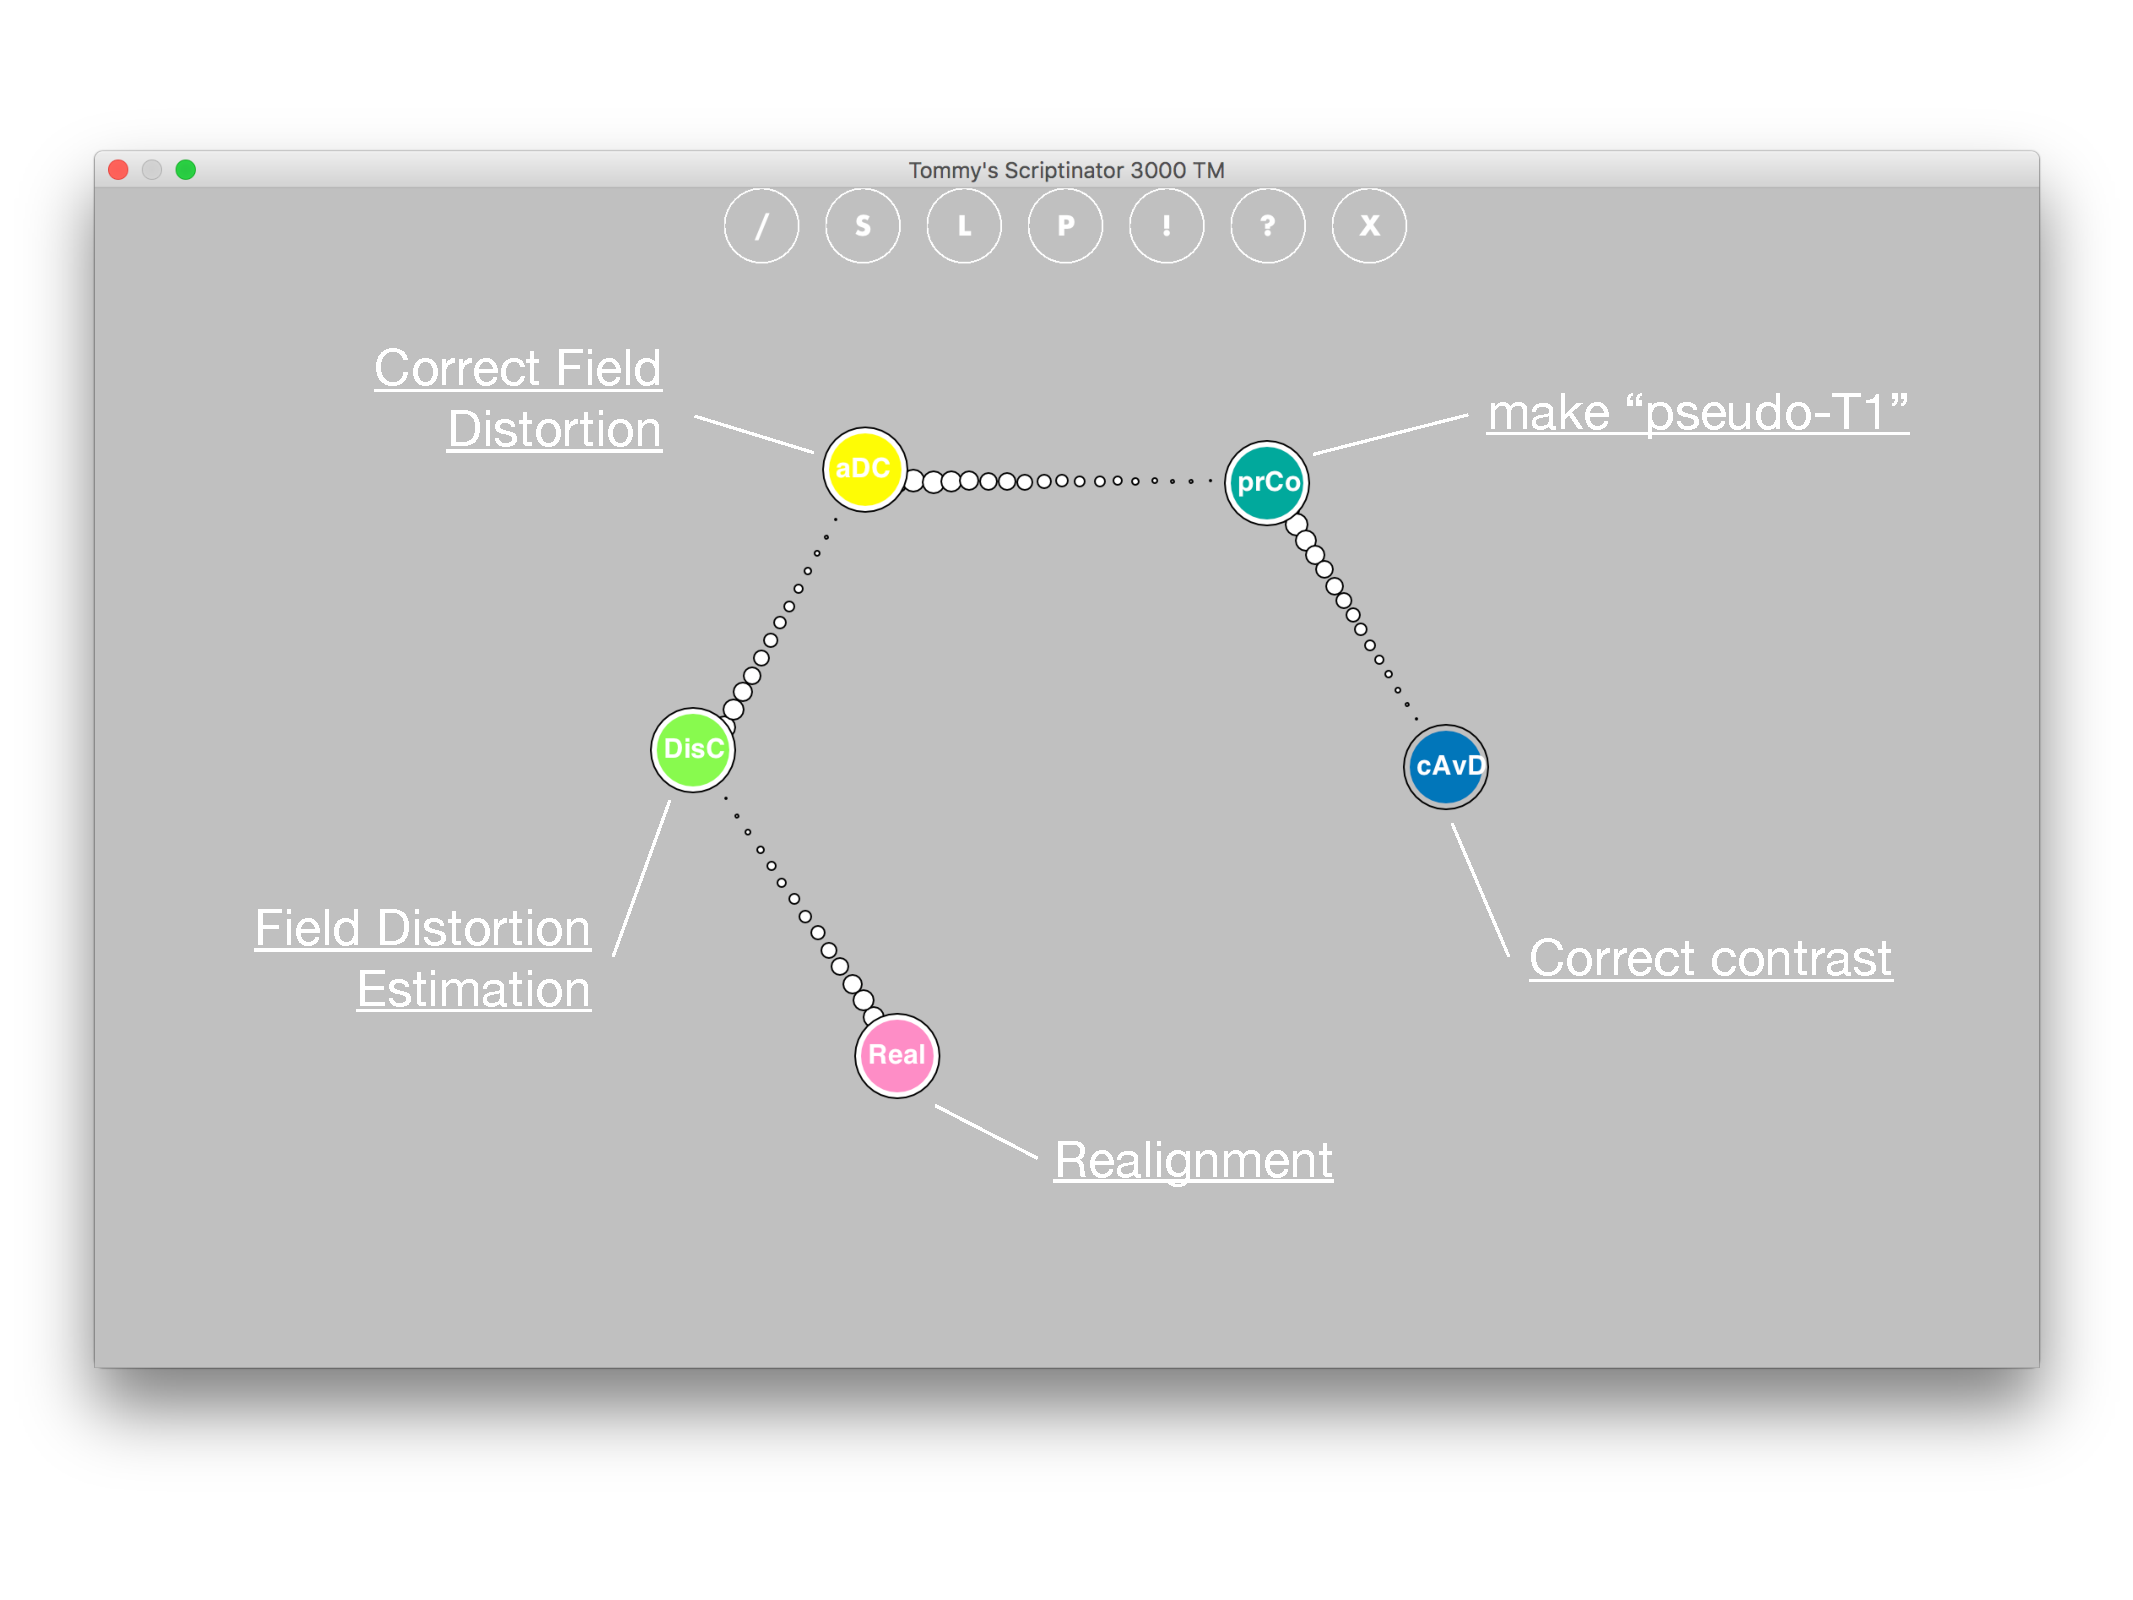
\includegraphics[width=\textwidth]{preproc-pipe}
\caption[Pre-processing Pipeline]{Example pipeline for the pre-processing, using Tommy's Scriptinator 3000 TM: preprocessing.pipe}
\end{center}
\end{figure}

\begin{figure}[h]
\begin{center}
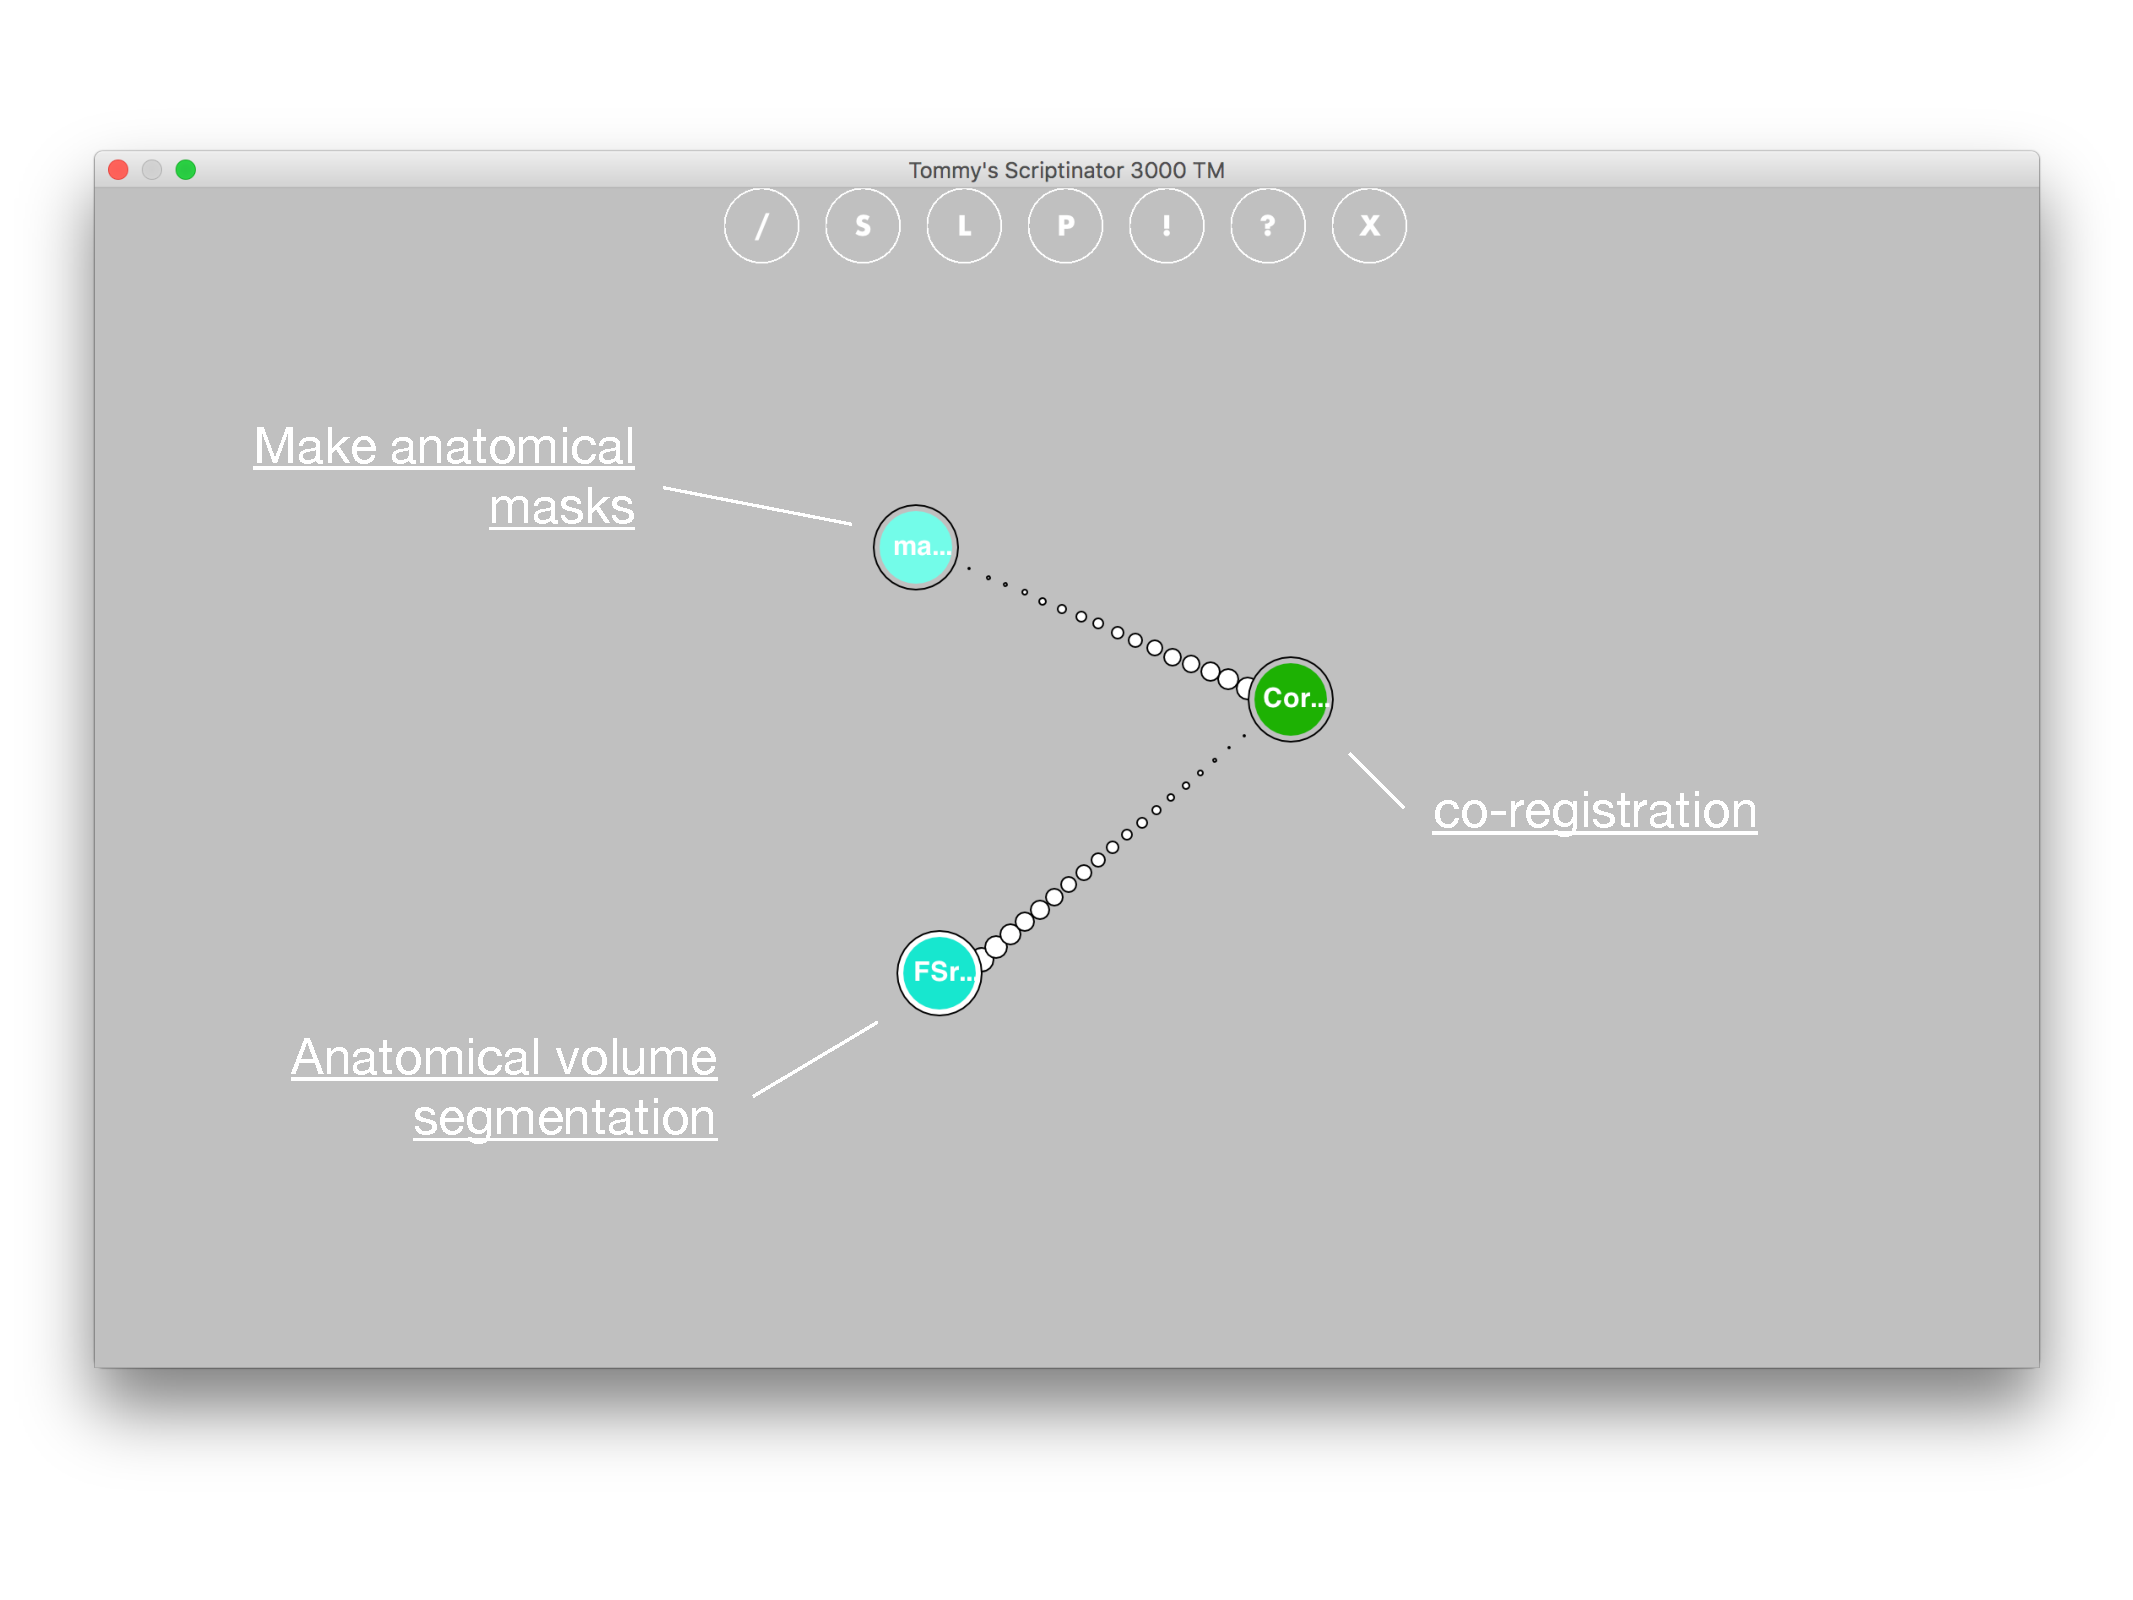
\includegraphics[width=\textwidth]{segment-pipe}
\caption[Segmentation Pipeline]{Example pipeline for the anatomical segmentation, using Tommy's Scriptinator 3000 TM: CoregistrationAndAnatMasks.pipe}
\end{center}
\end{figure}

\begin{figure}[h]
\begin{center}
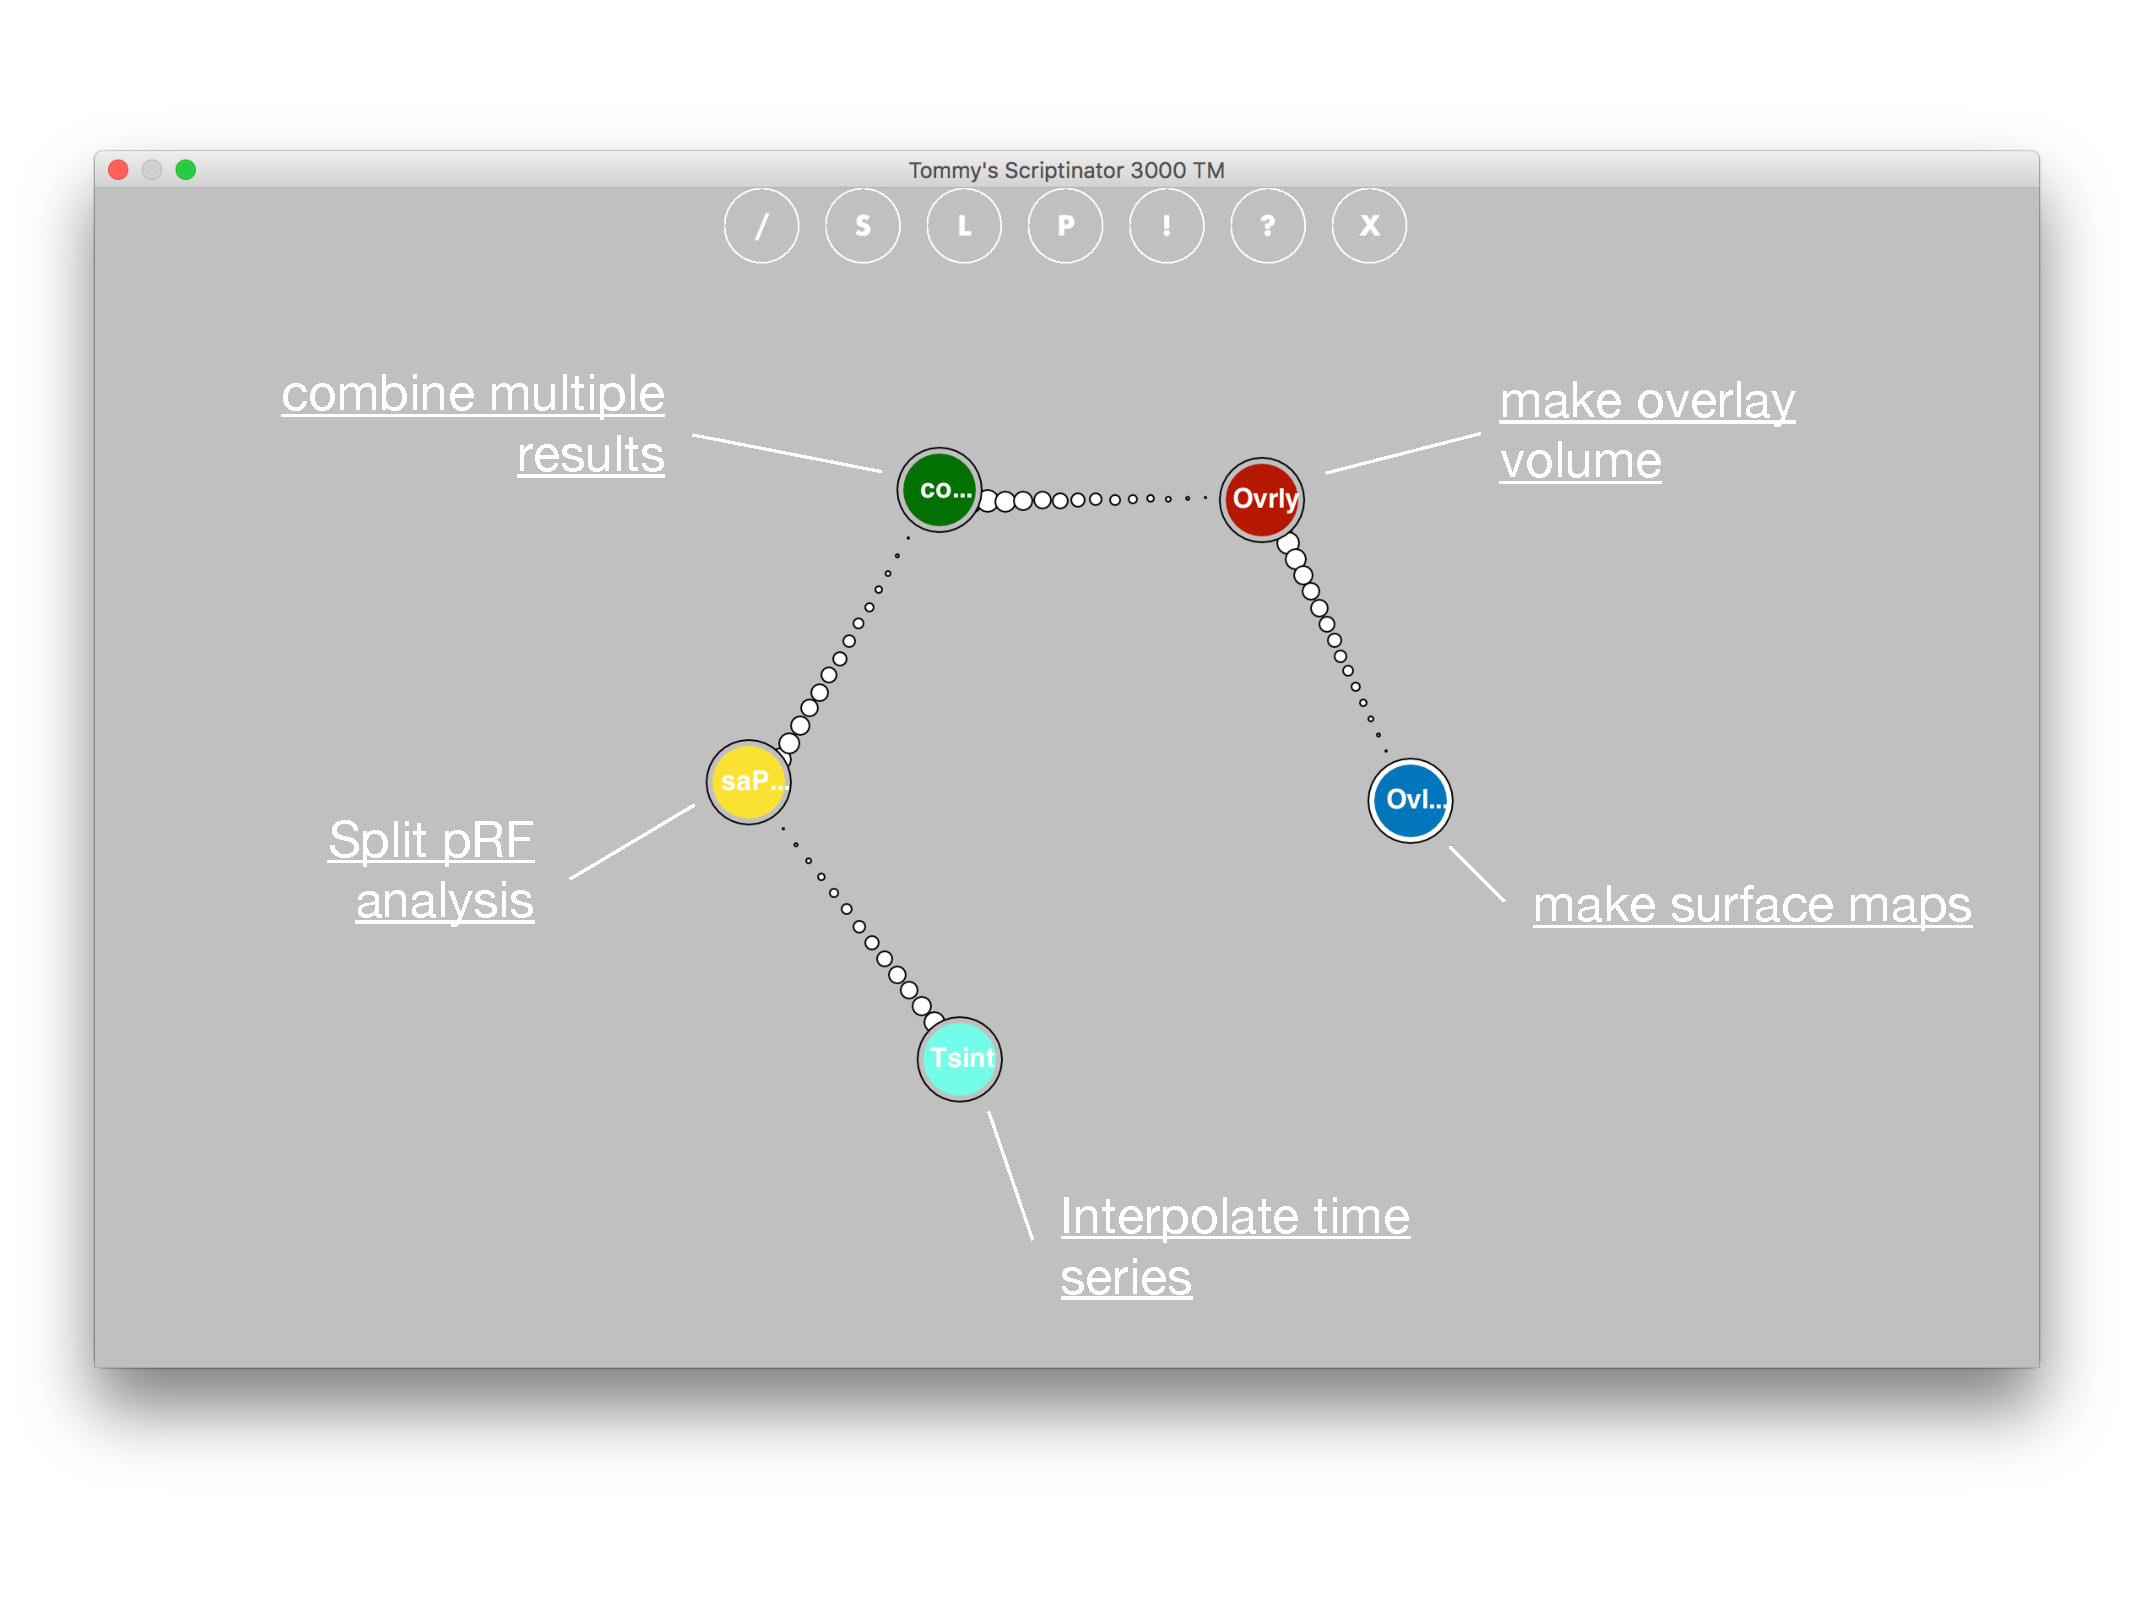
\includegraphics[width=\textwidth]{retino-pipe}
\caption[Retinotopy Pipeline]{Example pipeline for the retinotopy, using Tommy's Scriptinator 3000 TM: retinotopy.pipe}
\end{center}
\end{figure}

\begin{figure}[h]
\begin{center}
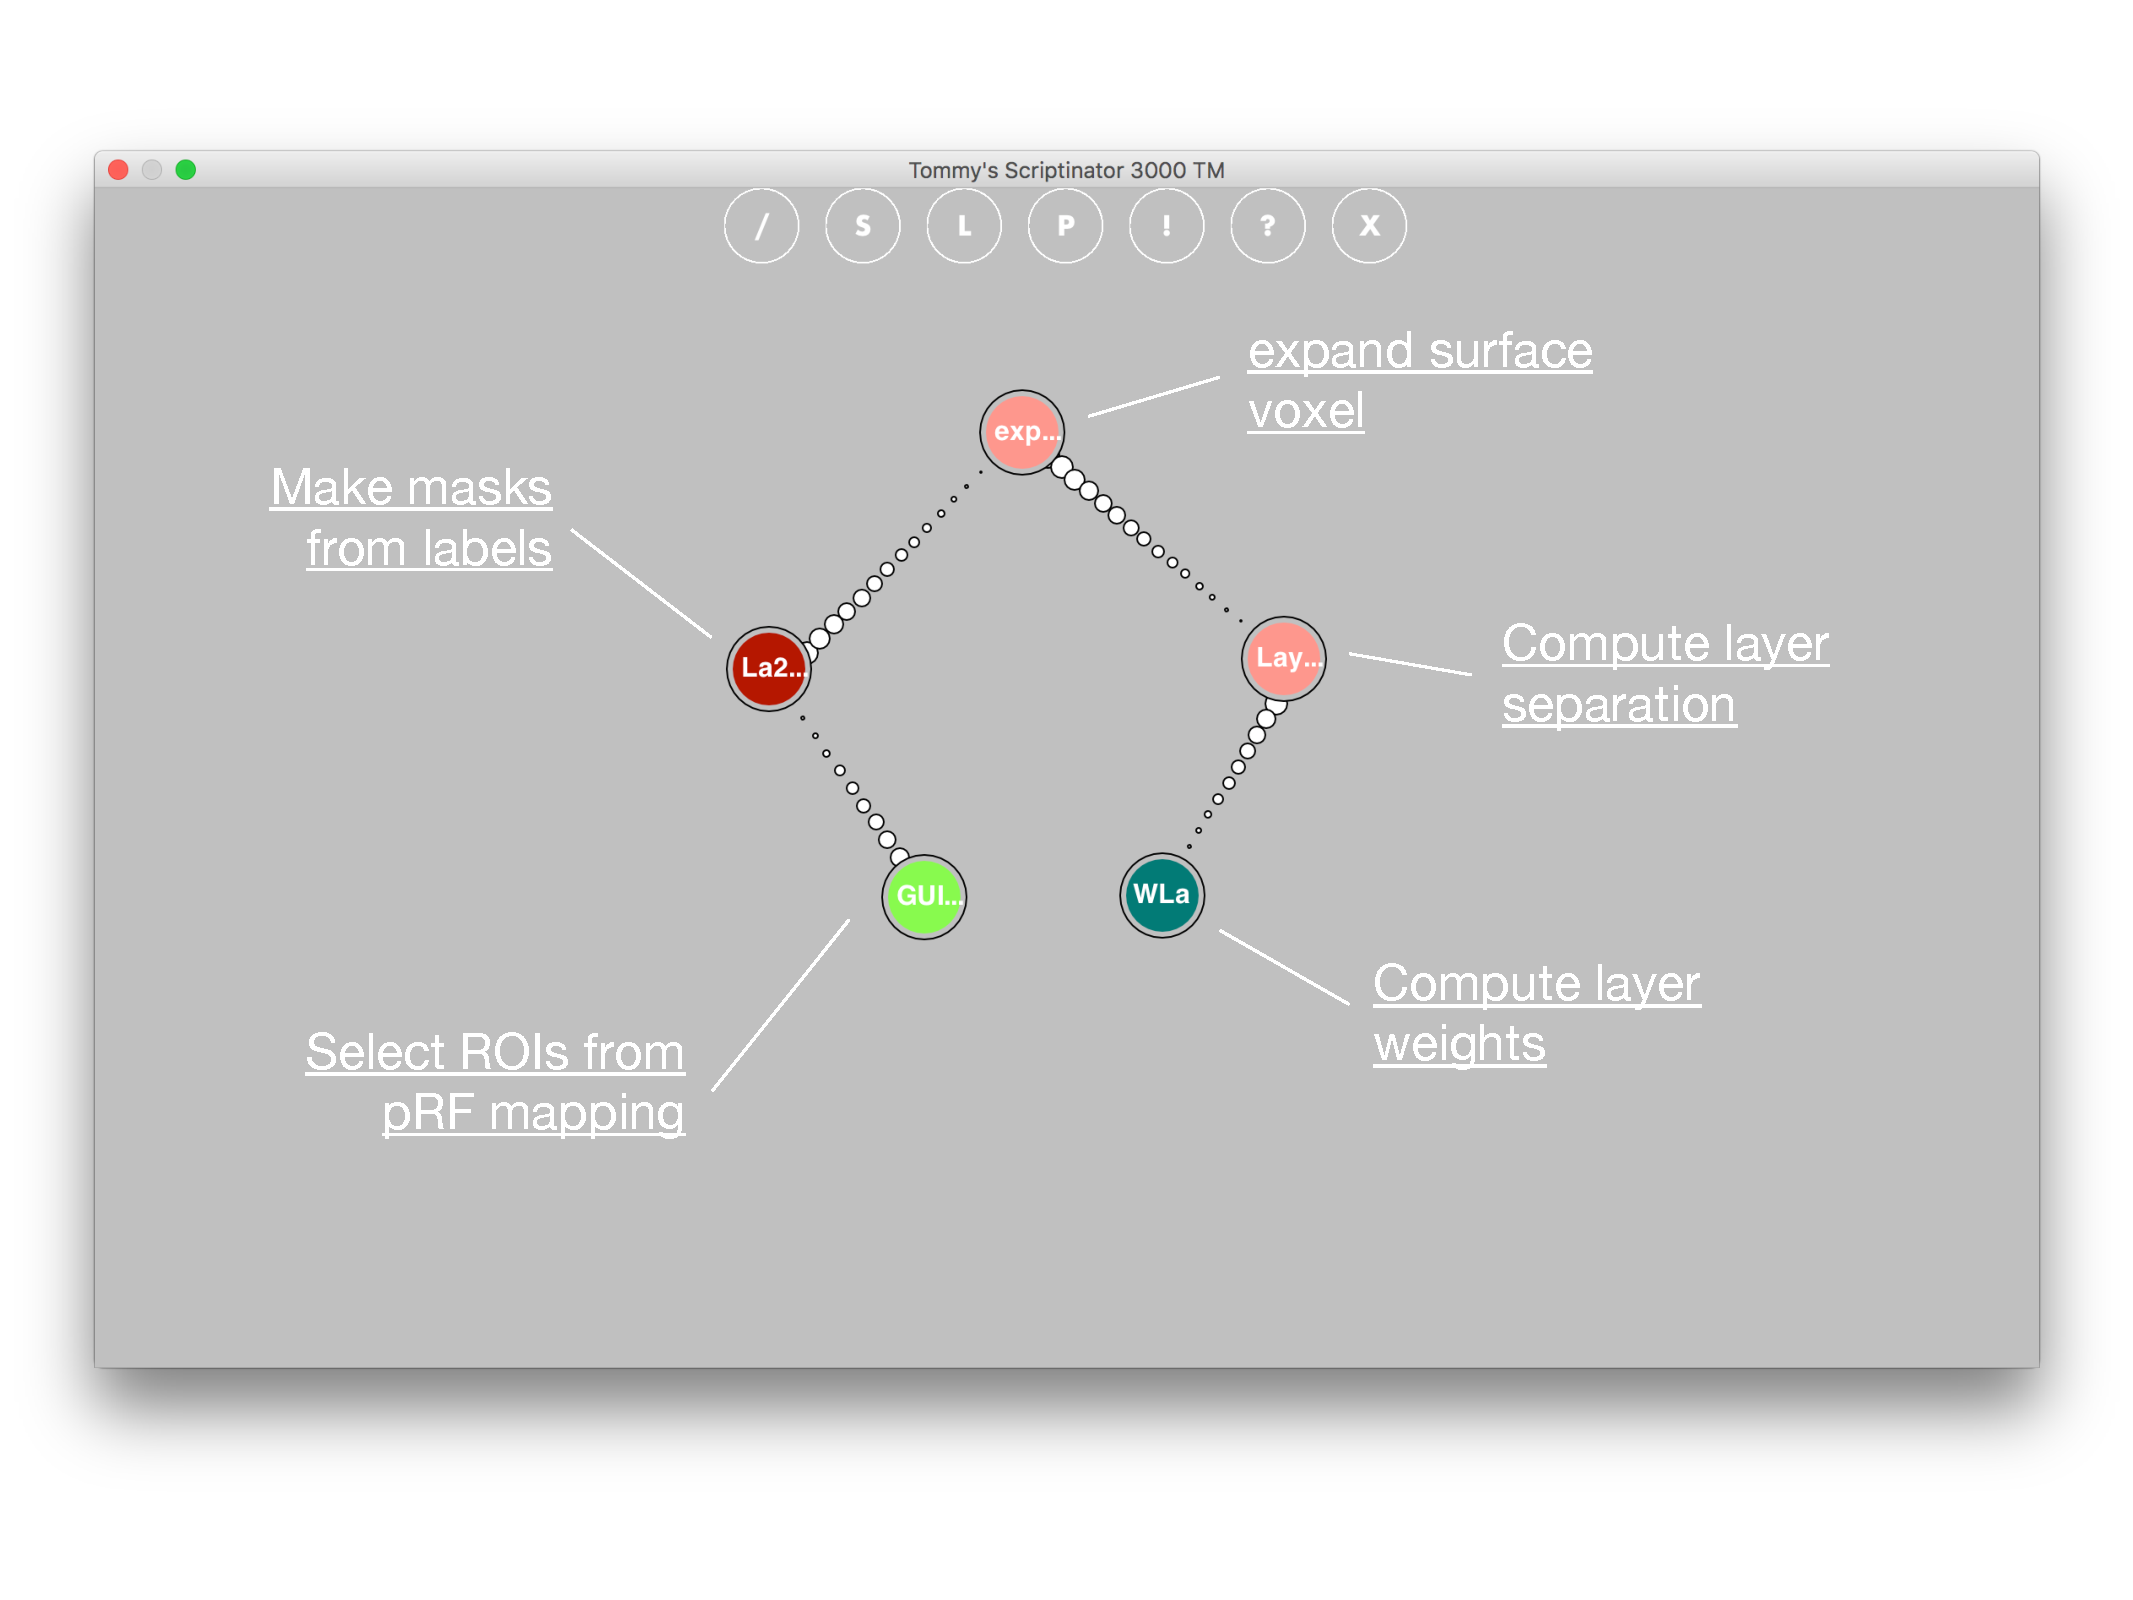
\includegraphics[width=\textwidth]{laminar-pipe}
\caption[Laminar definition Pipeline]{Example pipeline for the cortical layer definition, using Tommy's Scriptinator 3000 TM: laminar.pipe}
\end{center}
\end{figure}

\end{document}
